\documentclass[10pt,a4paper]{article}
\usepackage[margin=0.75in]{geometry}
\usepackage[T1]{fontenc}
\renewcommand{\rmdefault}{ptm}
\renewcommand{\ttdefault}{pcr}
\usepackage{amsmath,amssymb,booktabs,tabularx,array,graphicx}
\usepackage[hyphens]{url}
\usepackage[hidelinks]{hyperref}
\graphicspath{{figures/}}
\setlength{\parindent}{1em}
\setlength{\parskip}{4pt}
\setlength{\emergencystretch}{1em}
\renewcommand{\thetable}{S\arabic{table}}
\renewcommand{\thefigure}{S\arabic{figure}}
\renewcommand{\theequation}{S\arabic{equation}}
\newcolumntype{Y}{>{\raggedright\arraybackslash}X}
\newcommand{\tabnote}[1]{\par\smallskip{\footnotesize #1\par}}
\begin{document}
\begin{center}
{\Large\bfseries Focused Technical and Sensitivity Supplement\par}
\medskip
{\large Spatiotemporal Hybrid Ensemble Framework for Forecasting Respiratory Emergency Department Burden Using Syndromic Surveillance Data\par}
\medskip
Alexander Roque --- Department of Engineering\\
Isaac Osunmakinde --- Department of Computer Science\\
Norfolk State University, Norfolk, VA, USA\\
\smallskip ICCA 2026, Paper 1571299889 --- November 15, 2026
\end{center}

\noindent This companion provides implementation detail and archived evaluation evidence for the six-page working manuscript. No experiment was added, no learner was refitted, and no saved prediction or heat-map asset was changed. Experiments 1--3 denote NSSP, contemporary ILINet, and historical ILINet. Primary hybrid $R^2$ values are 0.599, 0.890, and 0.895. NSSP now leads with one equally weighted observation per HSA-week; its original reporting-record-weighted $R^2=0.671$ remains a secondary comparison. This post-review reporting amendment uses the existing geographic rescoring in Section S4, not a prespecified validation redesign. Training and model selection retain their original record weighting. Errors are in percentage points; comparisons are descriptive, without confidence intervals or significance claims.

\section*{S1. Additional feature, fitting, and cluster-profile details}
\label{sec:S1}
\subsection*{Availability-aligned feature construction}
For reporting unit $r$ and target week $t$, $y_{r,t}$ is the combined respiratory emergency-department visit percentage in NSSP or unweighted outpatient ILI percentage in ILINet. The newest surveillance observation used to forecast $y_{r,t}$ is from completed week $t-1$. Within each ordered reporting series,
\begin{equation}
\operatorname{lag}_k(r,t)=y_{r,t-k},\qquad k\in\{1,2,3\}.
\label{eq:lags}
\end{equation}
The three preceding target observations also give
\begin{equation}
\operatorname{RollingMean}_3(r,t)=\frac{1}{3}\sum_{i=1}^{3}y_{r,t-i},
\label{eq:mean}
\end{equation}
\begin{equation}
\operatorname{RollingStd}_3(r,t)=\sqrt{\frac{1}{2}\sum_{i=1}^{3}
\left[y_{r,t-i}-\operatorname{RollingMean}_3(r,t)\right]^2}.
\label{eq:std}
\end{equation}
The denominator 2 in (\ref{eq:std}) is the sample-standard-deviation convention used by the implementation. Annual phase is
\begin{equation}
\operatorname{WeekSin}(t)=\sin\!\left(\frac{2\pi w_t}{52}\right),\qquad
\operatorname{WeekCos}(t)=\cos\!\left(\frac{2\pi w_t}{52}\right),
\label{eq:season}
\end{equation}
where $w_t$ is the source epidemiological-week number. Under this fixed denominator, Week 53 has the same phase as Week 1. This convention applies to 2025-W53 in contemporary ILINet and describes annual seasonality, not multi-decadal cycles. The seasonal-naive benchmark is a 52-observation shift, not a calendar-week join.

NSSP auxiliary inputs are \nolinkurl{percent_visits_covid_lag_1}, \nolinkurl{percent_visits_influenza_lag_1}, and \nolinkurl{percent_visits_rsv_lag_1}. ILINet uses \nolinkurl{NUM. OF PROVIDERS_lag_1}. These are created by shifting their source variables one observation within the reporting series. Current target-week outcomes, component shares, smoothed values, and trends are excluded. Source series in the audited snapshots are contiguous weekly; every final-test lag-1 interval is seven days. This does not establish that values would have been published without delay or later revision.

Missing-value markers are converted to unavailable values. Rows missing the target or a required engineered feature are excluded; no median imputation or geographic-category encoding is used. Weekly chronology is preserved across geographic records. Each experiment has its own fitted preprocessing objects, learners, weights, and classical models; no NSSP-fitted object is transferred to ILINet.

\clearpage
\subsection*{Fitting boundary and cluster profiles}
Table~\ref{tab:fitting} distinguishes chronological ensemble validation from full-pretest refitting. The MLP's internal stopping subset is a random 15\% of the rows supplied to the current fit, using seed 42. It is not a separate chronological validation window. During weight estimation it is drawn only from the earlier fitting segment; during final refitting it is drawn only from the complete pre-test history. Final-test rows never enter that stopping subset.

\begin{table}[!ht]
\centering\small
\caption{Objects fitted or held fixed at each evaluation stage.}
\label{tab:fitting}
\begin{tabularx}{\textwidth}{@{}p{0.18\textwidth}YY@{}}
\toprule
Stage & Fitted / estimated & Held out or held fixed\\
\midrule
Chronological fitting & Scaler, K-means, RF, GBR, and MLP on earlier pre-test weeks & Latest 20\% of pre-test weeks reserved for weight estimation; final test excluded\\
Validation & Learner validation MSE determines normalized inverse-MSE weights; classical candidates ranked by pooled RMSE then MAE & Fitting-segment preprocessing and learners are not refitted to validation rows for these predictions\\
Full-pretest refit & New scaler, centroids, and learners on complete pre-test history; per-series classical fits with selected orders & $K=4$, learner settings, ensemble weights, and classical orders fixed before final-test scoring\\
Rolling final test & Completed observations become lagged inputs; classical states update without parameter refitting & No final-test outcomes fit preprocessing, centroids, learner parameters, weights, or classical orders\\
\bottomrule
\end{tabularx}
\end{table}

For K-means, every input feature is centered and scaled using statistics from the current fitting segment. K-means is fitted in the full standardized feature space; one-hot cluster indicators are appended to those features. Candidate $K=2,\ldots,8$ diagnostics use the chronological NSSP fit segment only. The largest silhouette was 0.484 at $K=2$; the largest elbow distance occurred at $K=4$, whose silhouette was 0.308. $K=5$ gave 0.321, while at $K=8$ the smallest cluster contained only 19 fit observations. Thus $K=4$ is an elbow-supported parsimonious choice, not the silhouette or final-test optimum.

After fixing $K$, scaling and centroids were refitted on the complete 183,384-row NSSP pre-test history. Table~\ref{tab:profiles} gives the resulting profiles. ``Burden'' is the mean standardized centroid across target lags 1--3 and the rolling mean; variability is the rolling standard deviation. Phase week is an approximate description of the sine/cosine centroid, not a calendar boundary. The two-dimensional principal component analysis (PCA) in Fig.~\ref{fig:clusters} is for display only; its first two components explain 69.7\% of variance.

\begin{table}[!ht]
\centering\small
\caption{NSSP cluster profiles after full-pretest refitting ($N=183,384$).}
\label{tab:profiles}
\setlength{\tabcolsep}{4pt}
\begin{tabular}{lrrrrrrrr}
\toprule
Cluster & Rows & Share & Burden $z$ & Variability $z$ & COVID $z$ & Flu $z$ & RSV $z$ & Phase week\\
\midrule
0 & 49,367 & 26.9\% & 0.578 & 0.295 & 0.548 & 0.347 & 0.371 & 2.4\\
1 & 71,785 & 39.1\% & -0.627 & -0.388 & -0.623 & -0.450 & -0.416 & 17.3\\
2 & 45,825 & 25.0\% & -0.430 & -0.276 & 0.008 & -0.457 & -0.172 & 40.3\\
3 & 16,407 & 8.9\% & 2.214 & 1.584 & 1.059 & 2.211 & 1.188 & 51.7\\
\bottomrule
\end{tabular}
\tabnote{COVID, influenza, and RSV columns describe one-week-lagged component shares. Shares are rounded and need not sum to exactly 100\%.}
\end{table}

Cluster 1 is the largest lower-burden regime; Cluster 2 is also below average in burden but has near-average lagged COVID-19 share. Cluster 0 is moderately elevated. Cluster 3 is the smallest, highest-burden regime, particularly for lagged influenza. These are descriptive feature-space profiles, not causal classes or fixed geographic regions. Full-pretest silhouettes are 0.303 for NSSP, 0.262 for contemporary ILINet, and 0.269 for historical ILINet, indicating overlap rather than sharply separated epidemiological states.

\clearpage
\subsection*{Cluster-selection visualization}
\begin{figure}[!ht]
\centering
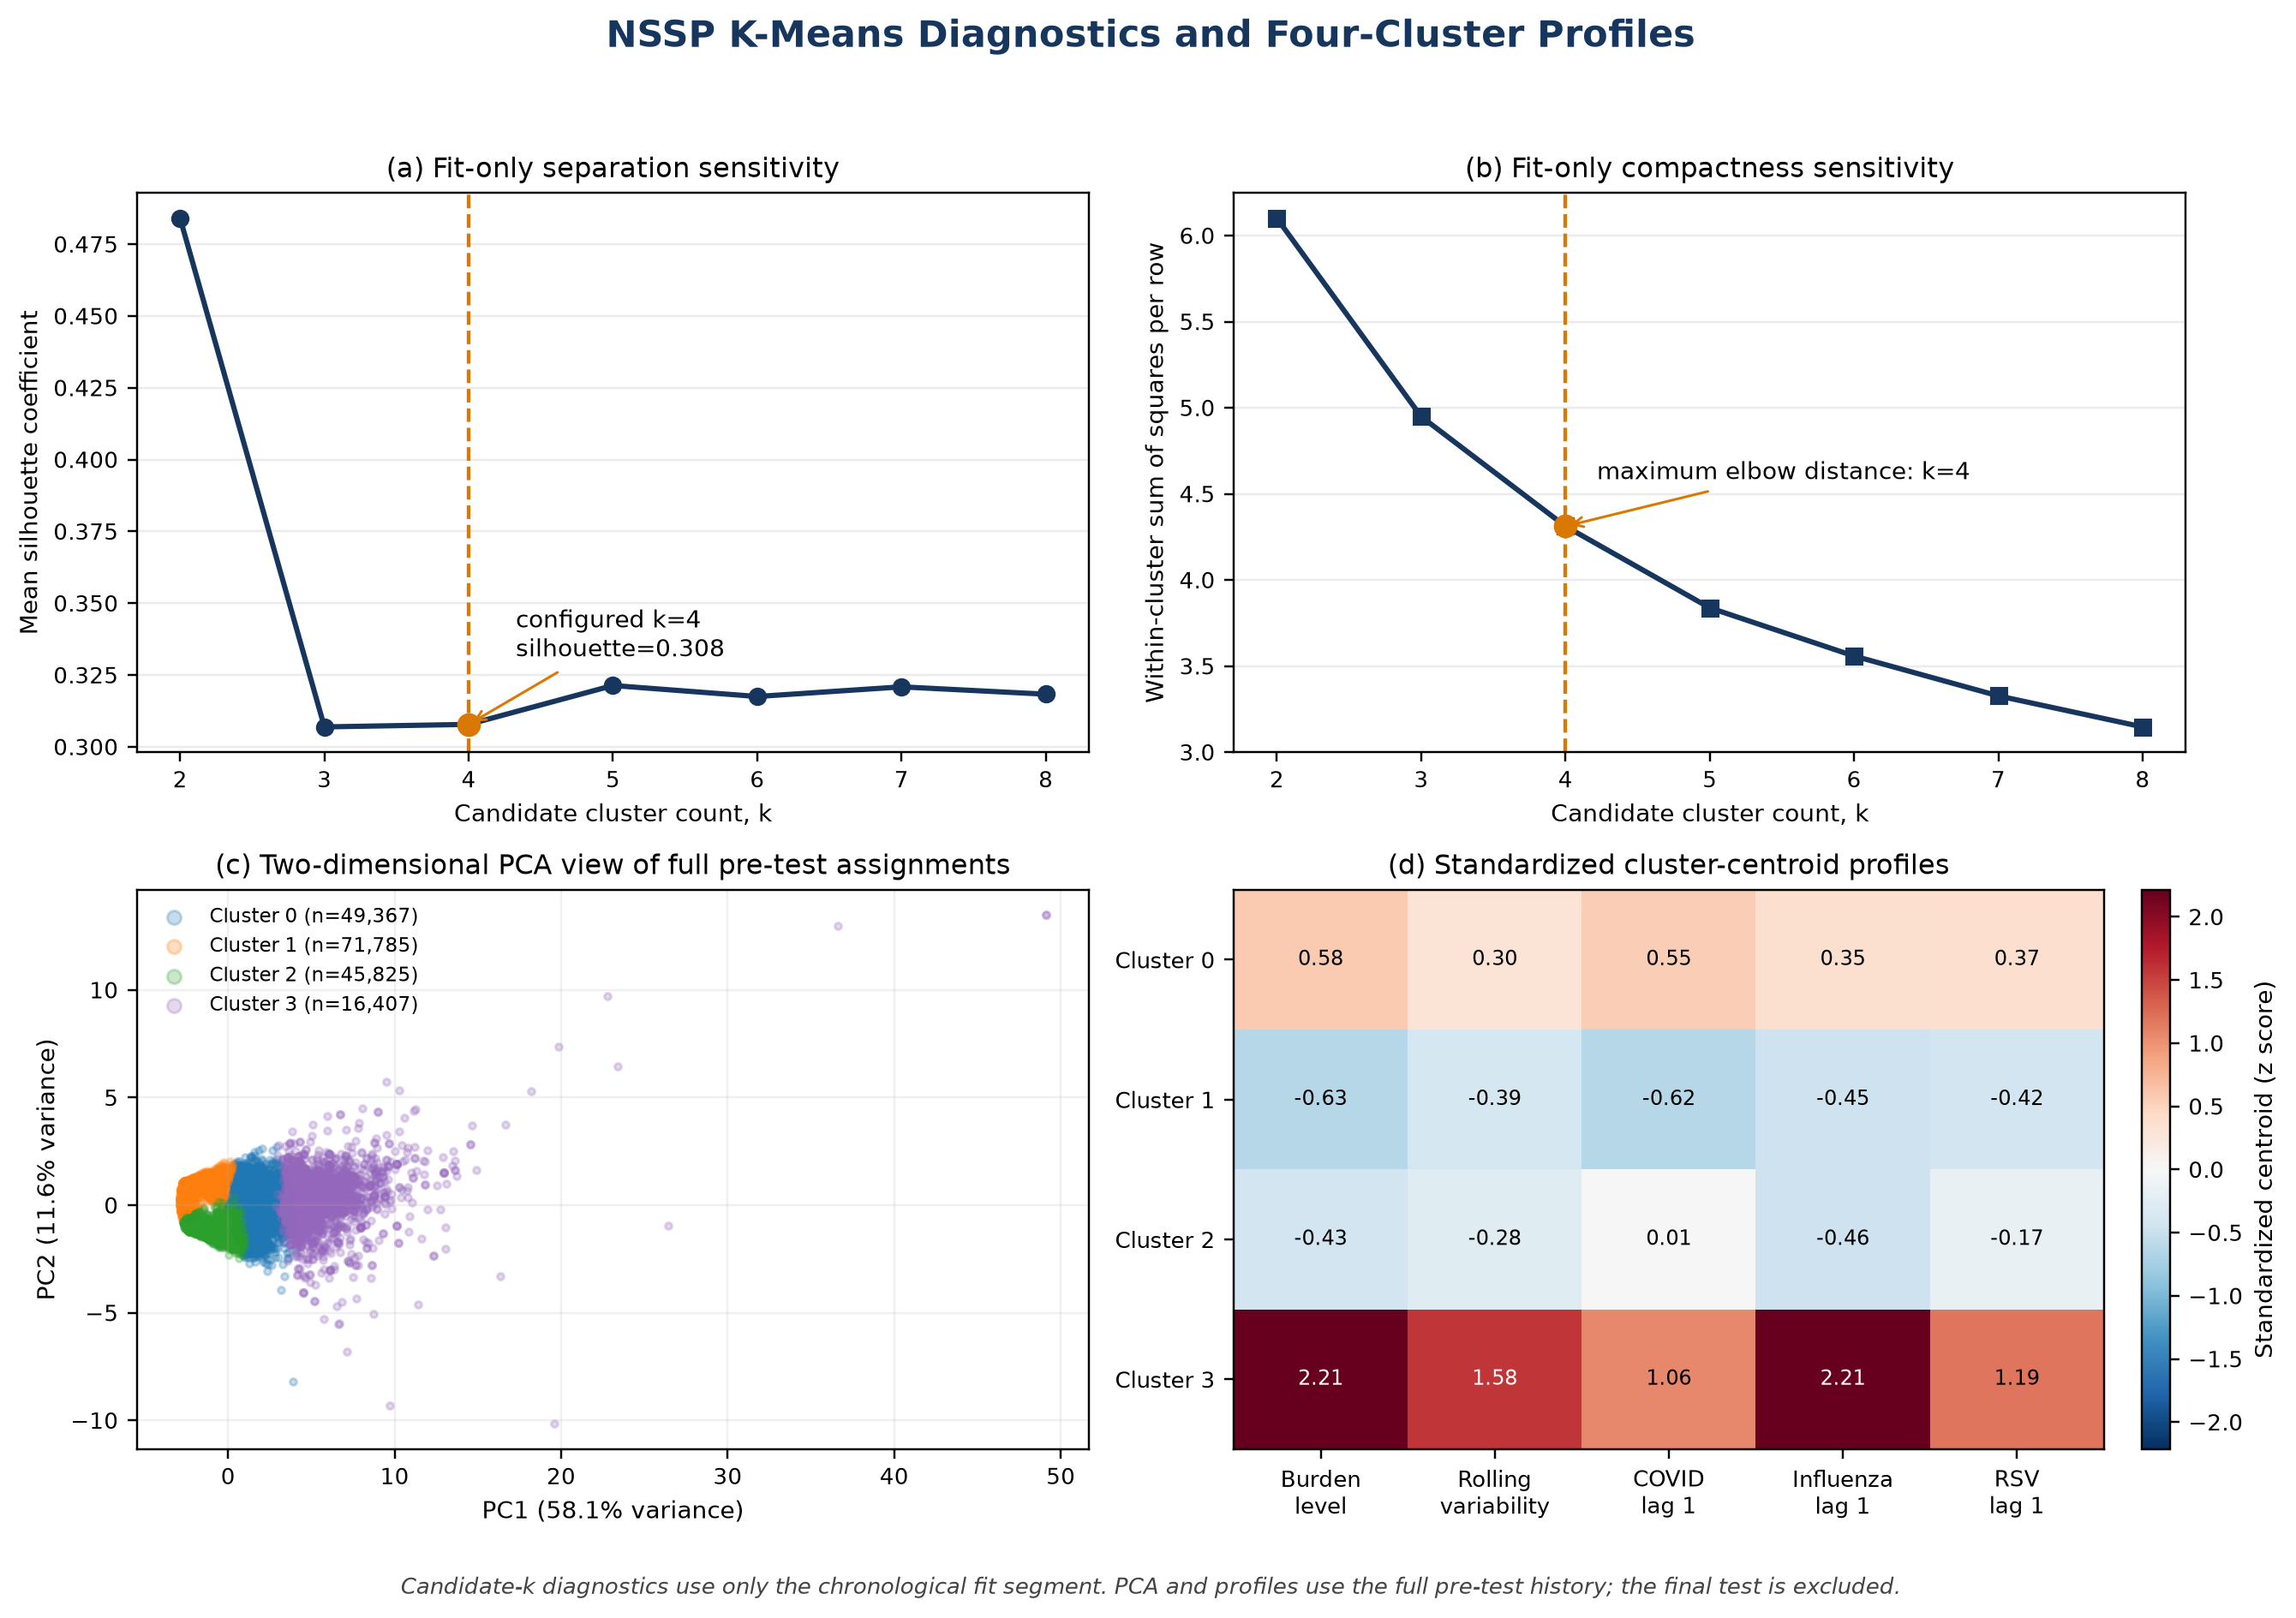
\includegraphics[width=\textwidth]{fig02.png}
\caption{NSSP clustering diagnostics. Candidate-$K$ compactness and silhouette use the chronological fit segment only. The PCA projection and centroid profiles describe complete pre-test history after $K$ is fixed; test outcomes are excluded. PCA is for display, not the space in which K-means was fitted. Cluster indicators describe overlapping surveillance regimes, not causal disease classes or fixed regions.}
\label{fig:clusters}
\end{figure}

\clearpage
\subsection*{Fixed learner settings and stopping procedure}
Table~\ref{tab:settings} reports the explicit feature and learner settings retained by the implementation. They are fixed design choices, not the outcome of an exhaustive learner-hyperparameter search. The archived software environment identifies the library versions governing unlisted estimator defaults. During each fitting phase, the RF, GBR, and MLP regressors are trained separately on the same augmented feature matrix. Validation predictions determine ensemble weights; the selected weights are then held fixed while new preprocessing objects and learners are fitted on complete pre-test history.

\begin{table}[!ht]
\caption{Availability-aligned features and fixed learning settings.}
\label{tab:settings}\centering\footnotesize
\begin{tabularx}{\textwidth}{@{}p{0.18\textwidth}p{0.43\textwidth}Y@{}}
\toprule
Component & Implemented definition or setting & Purpose / information boundary\\
\midrule
Target history & Target lags 1, 2, and 3, constructed within each series & Most recent three completed weeks\\
Rolling summaries & Mean and sample standard deviation of those three values & Recent level and variability; no target-week value\\
Annual phase & $\sin(2\pi w/52)$ and $\cos(2\pi w/52)$ for target-week number $w$ & Known target-week calendar; Week 53 repeats Week 1 phase\\
Auxiliary inputs & NSSP: COVID-19, influenza, and RSV shares at $t-1$; ILINet: provider count at $t-1$ & Dataset-specific completed-week signals\\
Structural context & Standardized inputs; four one-hot K-means indicators; 10 initializations & Scaler and centroids fitted within each training segment\\
Random forest & 150 trees; unlimited depth; minimum split 2; minimum leaf 1; one job & Bootstrap aggregation of regression trees\\
Gradient boosting & 150 estimators; maximum depth 3; learning rate 0.05 & Sequential regression of prediction errors\\
Multilayer perceptron & Hidden layers (32,16); ReLU; Adam; regularization 0.0001; initial learning rate 0.001; maximum 300 iterations & Compact nonlinear learner; random 15\% internal stopping subset\\
Stopping and weighting & MLP: 20 epochs without score improvement of 0.0001; ensemble: inverse-MSE on latest 20\% of pre-test weeks & Internal stopping differs from outer chronological weight validation\\
Refit and reproducibility & Fix weights/orders; rebuild fitted objects on complete pre-test history; seed 42 & Final-test outcomes excluded from parameter estimation\\
\bottomrule
\end{tabularx}
\end{table}

With early stopping enabled, the MLP monitors its internal validation score with tolerance $10^{-4}$ and \nolinkurl{n_iter_no_change=20}, subject to \nolinkurl{max_iter=300}. Its random 15\% stopping subset comes only from the rows supplied to that particular fit. It is distinct from the later chronological validation interval used to calculate ensemble MSE. The implementation parameters are retained in \nolinkurl{src/common_config.py}; fitting and weighting are implemented in \nolinkurl{src/common_models.py}.

\clearpage
\subsection*{Classical candidate search, fitting, and convergence}
The bounded nonseasonal grid comprises ARIMA$(1,0,0)$, ARIMA$(0,1,1)$, and ARIMA$(1,1,0)$. The annual grid combines nonseasonal orders $(1,0,0)$, $(2,0,0)$, or $(1,0,1)$ with seasonal order $(1,0,0)_{52}$. A constant term is used for the undifferenced candidates; the differenced nonseasonal candidates have no trend term. Each candidate is fitted separately to each reporting series. Within each experiment and family, pooled chronological-validation RMSE, then MAE, selects one common order from candidates with at least 95\% prediction coverage.

Models use the statsmodels SARIMAX implementation with L-BFGS optimization and a maximum of 75 iterations. Stationarity and invertibility enforcement are disabled, and the scale parameter is concentrated out. After selection, the chosen order is fitted anew to each series' complete pre-test history. Final-test forecasts are one-step predictions from filtering with those fixed parameters: completed observations update the state, but test outcomes do not refit parameters. The classical models use target histories without the hybrid's auxiliary features.

\begin{table}[!ht]
\centering\small
\caption{Selected classical orders and archived final-test diagnostics.}
\label{tab:classical}
\begin{tabularx}{\textwidth}{@{}lYYrrr@{}}
\toprule
Experiment & ARIMA order & SARIMA order & Test rows & Coverage & Convergence\\
\midrule
1: NSSP & $(1,0,0)$ & $(1,0,0)\times(1,0,0)_{52}$ & 47,534 & 100\% / 100\% & 99.3\% / 99.9\%\\
2: Contemporary ILINet & $(0,1,1)$ & $(1,0,1)\times(1,0,0)_{52}$ & 1,774 & 100\% / 100\% & 100\% / 100\%\\
3: Historical ILINet & $(1,1,0)$ & $(2,0,0)\times(1,0,0)_{52}$ & 2,808 & 100\% / 100\% & 100\% / 98.1\%\\
\bottomrule
\end{tabularx}
\tabnote{Pairs report ARIMA / SARIMA. These archived diagnostics retain original prediction-record counts, not the 13,356 HSA-week primary NSSP scoring units. Coverage is the fraction of required test rows with predictions; convergence is the fraction of fitted reporting series for which the optimizer reported convergence. NSSP counts are 2,248/2,264 for ARIMA and 2,261/2,264 for SARIMA. Each ILINet experiment has 54 fitted series; historical SARIMA converged for 53/54. Finite forecasts from nonconverged fits remain in the scores, so full coverage is not full convergence.}
\end{table}

Seasonal differencing was screened separately for NSSP, not assumed unsuccessful in every surveillance setting. Three $D=1$ candidates, $(1,0,0)\times(0,1,1)_{52}$, $(0,1,1)\times(0,1,1)_{52}$, and $(1,1,0)\times(0,1,1)_{52}$, were evaluated on the same deterministic 120-series validation cohort. All produced forecasts but had 0\% optimizer convergence at 75 iterations. The accuracy-competitive $(1,0,0)\times(0,1,1)_{52}$ candidate was retested on 60 series with 300 iterations and still had 0\% convergence. These candidates were not promoted to the 2,264-series NSSP run or its final test. This documents a computational and search boundary, not a claim that seasonal differencing or SARIMA is generally inferior.

Candidate definitions and fitting code are archived under \nolinkurl{benchmarks/sarima/}. The preserved results under \nolinkurl{results/reference/classical/} include the NSSP full-run completion records and methodological decision, the ILINet run summaries, and the nonseasonal ARIMA extension report. No candidate selection, fitting, or diagnostic calculation was repeated to prepare this supplement.

\clearpage
\section*{S2. Auxiliary-lag development history}
\label{sec:S2}
The retained auxiliary configuration uses one previous observation: COVID-19, influenza, and RSV percentages in NSSP and provider count in ILINet. Target-history features retain three lags in both configurations. Thus, ``[1]'' and ``[1,2,3]'' below refer only to auxiliary-variable lags, not to the target's lag set.

The archived NSSP comparison used three expanding rolling-origin windows and the original reporting-record weighting, not HSA-week scoring. Each validation window contained 10 epidemiological weeks and 22,640 records. Training/validation boundaries were 2022-W42--2023-W40 / 2023-W41--W50 (115,464 training records), 2022-W42--2023-W50 / 2023-W51--2024-W08 (138,104), and 2022-W42--2024-W08 / 2024-W09--W18 (160,744). Table~\ref{tab:rolling} reports saved, unweighted means across these windows, not pooled final-test scores. Auxiliary lags [1,2,3] had the lowest mean validation RMSE.

\begin{table}[!ht]
\centering
\caption{Archived NSSP rolling-origin hybrid comparison across three windows.}
\label{tab:rolling}
\begin{tabular}{lrrr}
\toprule
Auxiliary configuration & Mean MAE & Mean RMSE & Mean $R^2$\\
\midrule
{[1,2,3]} & 1.278290 & 1.905211 & 0.572740\\
Core only & 1.287427 & 1.934425 & 0.561527\\
{[1,2]} & 1.331049 & 1.955994 & 0.550609\\
{[1]} & 1.329988 & 1.961693 & 0.547841\\
\bottomrule
\end{tabular}
\end{table}

Both [1] and [1,2,3] were subsequently evaluated on the same final-test rows within each experiment (Table~\ref{tab:lags}). The single-lag model performed better for NSSP, whereas the three-lag variant had slightly lower RMSE in both ILINet experiments. The historical development process retained [1] as a parsimonious common configuration after these comparisons were available. The final test therefore cannot be described as untouched by all feature-set decisions. These development results are disclosed as a limitation, not recast as a new prospective selection exercise. No additional selection or model fitting was performed for this supplement.

\begin{table}[!ht]
\centering
\caption{Archived record-weighted final-test auxiliary-lag comparisons for the hybrid.}
\label{tab:lags}
\begin{tabular}{llrrrr}
\toprule
Experiment & Lags & $N$ & MAE & RMSE & $R^2$\\
\midrule
1: NSSP & [1] & 47,534 & 0.521423 & 0.803473 & 0.671288\\
 & [1,2,3] & 47,534 & 0.526204 & 0.813228 & 0.663258\\
2: Contemporary ILINet & [1] & 1,774 & 0.399268 & 0.716087 & 0.890186\\
 & [1,2,3] & 1,774 & 0.397852 & 0.710652 & 0.891846\\
3: Historical ILINet & [1] & 2,808 & 0.465868 & 0.833458 & 0.894556\\
 & [1,2,3] & 2,808 & 0.468131 & 0.832663 & 0.894757\\
\bottomrule
\end{tabular}
\tabnote{These saved development summaries are not newly fitted models. NSSP retains the original mixed-source record weighting; these are not primary HSA-week scores. Full-precision scores, fold boundaries, and source summaries accompany the archive.}
\end{table}

The conference paper separately reports record-weighted no-clustering and no-auxiliary-component ablations of the retained NSSP configuration. Their small conditional effects have not been evaluated on the primary HSA-week basis. Neither those tests nor the comparisons above separately remove the core target lags, rolling statistics, or seasonal indicators. Their individual contributions remain untested. Development-level holdout reuse is distinct from the within-run rule excluding test outcomes from parameter fitting.

\clearpage
\section*{S3. Ensemble-weight sensitivity}
\label{sec:S3}
The primary ensemble combines saved Random Forest (RF), Gradient Boosting Regressor (GBR), and multilayer perceptron (MLP) predictions using normalized inverse validation-MSE weights. The archived sensitivity replaces only those weights with $1/3$:
\begin{equation}
\widehat y_{\mathrm{equal}}=\frac{\widehat y_{\mathrm{RF}}+\widehat y_{\mathrm{GBR}}+\widehat y_{\mathrm{MLP}}}{3}.
\label{eq:equal}
\end{equation}
Component predictions, outcomes, and final-test rows are unchanged. The inverse-MSE prediction was reconstructed from its saved weights to verify the calculation. This archived sensitivity retains original record weighting for NSSP; it is not an HSA-week comparison. No weights were optimized on the test set, and no learners were retrained.

\begin{table}[!ht]
\centering
\caption{Saved normalized inverse validation-MSE weights.}
\label{tab:weights}
\begin{tabular}{lrrr}
\toprule
Experiment & RF & GBR & MLP\\
\midrule
1: NSSP & 0.309662 & 0.455147 & 0.235191\\
2: Contemporary ILINet & 0.369804 & 0.319095 & 0.311101\\
3: Historical ILINet & 0.331853 & 0.340901 & 0.327246\\
\bottomrule
\end{tabular}
\tabnote{The alternative assigns exactly $1/3$ to each learner. Validation errors and unrounded weights are retained in the machine-readable evidence.}
\end{table}

\begin{table}[!ht]
\centering
\caption{Archived record-weighted final-test rescoring with equal and inverse-MSE weights.}
\label{tab:equal}
\begin{tabular}{llrrrr}
\toprule
Experiment & Weighting & $N$ & MAE & RMSE & $R^2$\\
\midrule
1 & Inverse MSE & 47,534 & 0.521423 & 0.803473 & 0.671288\\
1 & Equal & 47,534 & 0.519484 & 0.801147 & 0.673189\\
2 & Inverse MSE & 1,774 & 0.399268 & 0.716087 & 0.890186\\
2 & Equal & 1,774 & 0.399246 & 0.716932 & 0.889926\\
3 & Inverse MSE & 2,808 & 0.465868 & 0.833458 & 0.894556\\
3 & Equal & 2,808 & 0.465858 & 0.833380 & 0.894576\\
\bottomrule
\end{tabular}
\end{table}

Equal weighting slightly reduced RMSE in record-weighted NSSP and the historical experiment; inverse-MSE weighting slightly reduced RMSE in contemporary ILINet. The largest absolute change was 0.002327 percentage points, in NSSP. These small, mixed differences do not establish general superiority of inverse-MSE weighting over a simple mean, nor its superiority on primary HSA-week scoring. They also do not establish temporal stability: each experiment contributes one validation-derived weight estimate, not estimates from repeated seasons or outbreak regimes. The primary weighting rule remains unchanged.

\subsection*{Interpretation and limits}
This check tests the numerical sensitivity of one retained ensemble to one alternative combination rule. It is not a comparison with every ensemble architecture, a new learner, or independent replications of a forecasting result. The three components share inputs and may have correlated errors. A new prospective test or repeated forecast-origin study would be needed to assess stability and uncertainty. Those analyses remain deferred.

\clearpage
\subsection*{Validation-derived ensemble weights}
\begin{figure}[!ht]
\centering
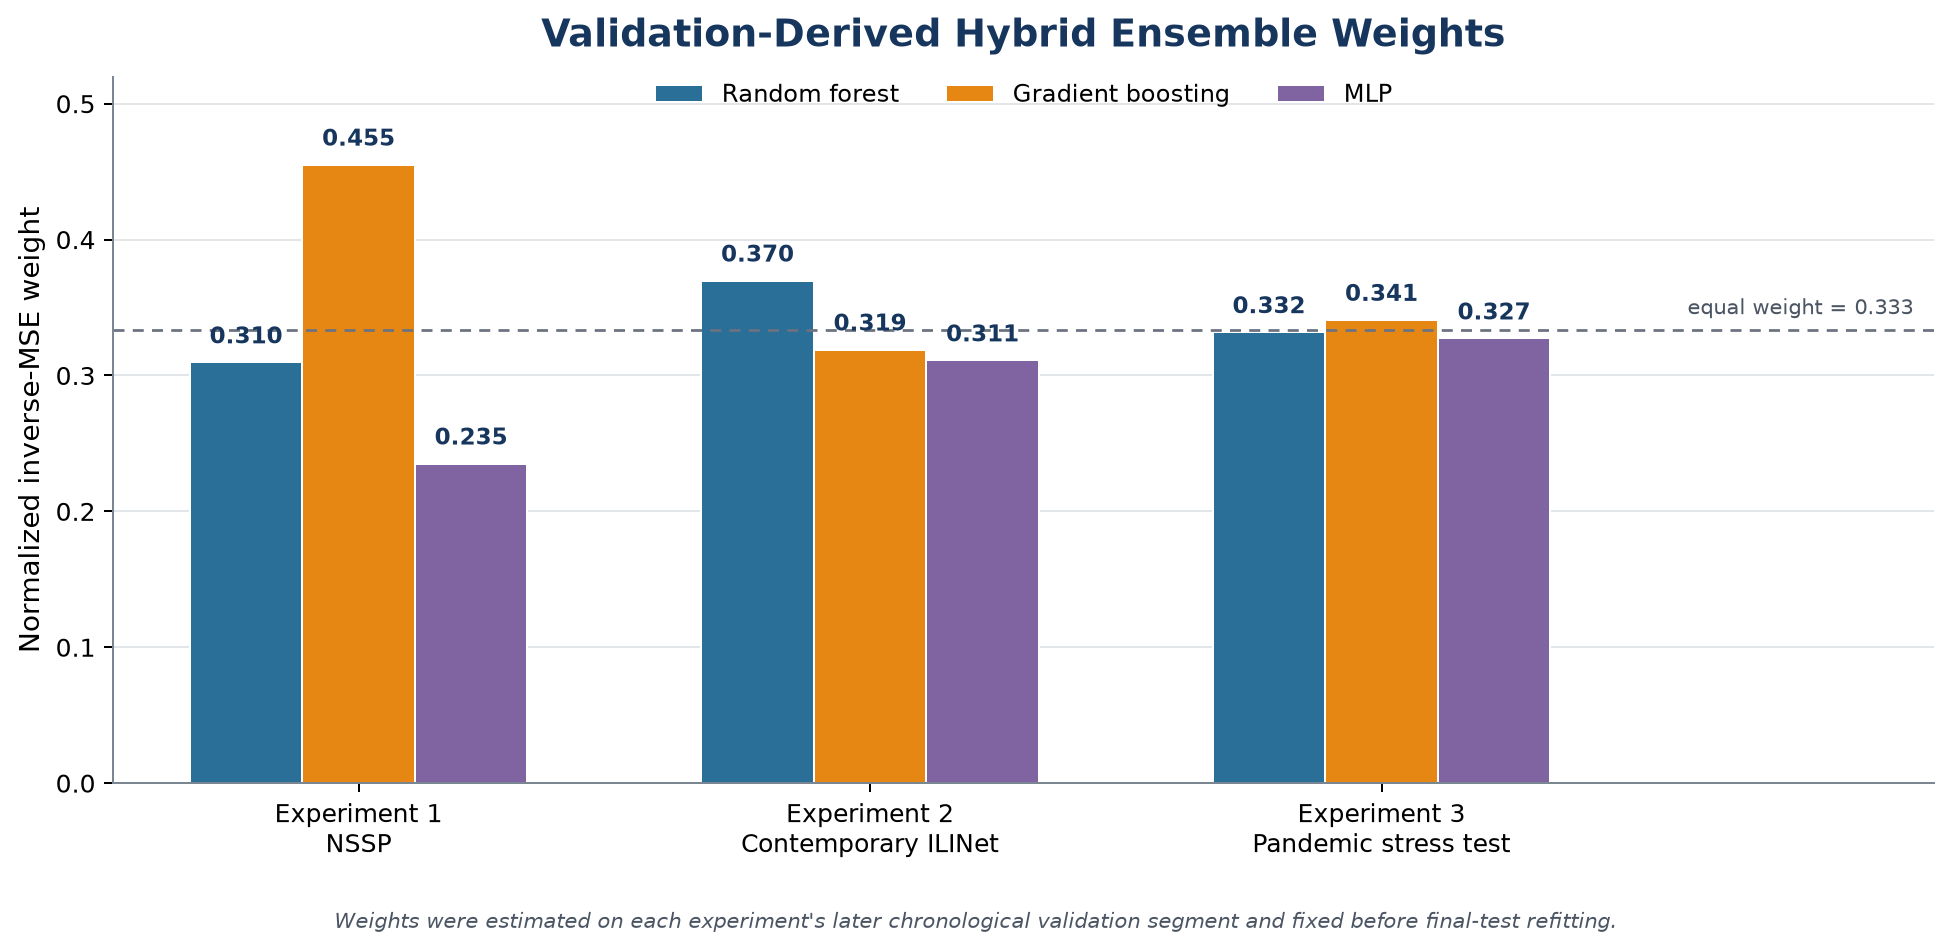
\includegraphics[width=\textwidth]{fig03.png}
\caption{Experiment-specific inverse-validation-MSE ensemble weights. Different weights reflect independently estimated validation errors, not demonstrated seasonal stability.}
\label{fig:weights}
\end{figure}

\clearpage
\section*{S4. Primary NSSP HSA-week scoring and record-weighted comparison}
\label{sec:S4}
The original 2,264 NSSP series keys combine 2,215 county-indexed keys carrying HSA values with 49 aggregate keys. A county name does not imply a county-specific measured outcome. The county-indexed records represent 636 HSAs, and multiple counties can share the same surveillance percentage. The aggregate keys comprise 48 state/DC keys and one national key. Table~\ref{tab:sources} describes the unchanged 2024-W19--W39 prediction cohort.

\begin{table}[!ht]
\centering
\caption{NSSP final-test source composition.}
\label{tab:sources}
\begin{tabular}{lrrrr}
\toprule
Source & Records & Series keys & HSA IDs & Weeks per key\\
\midrule
HSA, county-indexed key & 46,515 & 2,215 & 636 & 21\\
State/DC aggregate & 998 & 48 & --- & 11--21\\
National aggregate & 21 & 1 & --- & 21\\
\midrule
Original pooled total & 47,534 & 2,264 & --- & 11--21\\
\bottomrule
\end{tabular}
\tabnote{A series key is the pair (geography, county). Wyoming contributes 11 state-aggregate test rows; the other 48 aggregate keys contribute 21 each. These are record counts, not independent surveillance outcomes.}
\end{table}

Original record-weighted scoring gives every saved record equal weight, so an HSA represented by more county keys contributes more records. Primary NSSP scoring now uses the archived geographic calculation: restrict to HSA-source records, then average the observed target and each method's prediction within HSA--week. This yields 13,356 equally weighted HSA--weeks (636 HSAs over 21 weeks). Both targets and hybrid predictions agree within every HSA--week. Thus averaging removes repeated weighting without changing the hybrid forecasts. Of these units, 11,235 contain repeated county-key records, accounting for 44,394 of the 46,515 HSA-source records.

This post-review reporting amendment promotes an existing scoring-unit analysis; it was not prespecified. It changes the source cohort and evaluation weighting, not the fitted model, validation weights, selected classical orders, or prediction files. Repeated HSA contributions remain in the original training and validation process. The intermediate source-only row in Table~\ref{tab:cohorts} separates exclusion of state/national records from removal of repeated HSA-week weighting.

\begin{table}[!ht]
\centering
\caption{Hybrid performance under three NSSP scoring bases.}
\label{tab:cohorts}
\begin{tabular}{lrrrr}
\toprule
Scoring basis & $N$ & MAE & RMSE & $R^2$\\
\midrule
Primary: equal HSA--week means & 13,356 & 0.618219 & 0.972459 & 0.598622\\
Comparison: original mixed-source records & 47,534 & 0.521423 & 0.803473 & 0.671288\\
Intermediate: HSA-source county-key records & 46,515 & 0.526488 & 0.810114 & 0.669304\\
\bottomrule
\end{tabular}
\end{table}

The original mixed-source $R^2=0.671288$ changes only to 0.669304 after excluding state/national records. Most of the difference from primary HSA-week $R^2=0.598622$ therefore reflects repeated-record weighting, not aggregate-source exclusion. Equal HSA-week scoring better matches claims about distinct HSA surveillance outcomes, but neither the HSA-weeks nor the original records are asserted to be statistically independent. The original record-weighted score remains available for comparison. Geographic maps retain their original descriptive record weighting, not the primary HSA-week scoring basis.

\clearpage
\subsection*{All-method comparison and reproducibility}
Table~\ref{tab:geographic} applies identical HSA--week aggregation to all seven original methods and the two classical benchmarks. Classical predictions were matched one-to-one to the original geographic/epidemiological keys, and their targets were checked against the saved outcomes. All nine methods cover every unit in each displayed scoring cohort.

\begin{table}[!ht]
\centering\small
\caption{Primary NSSP HSA--week scores and original record-weighted comparison.}
\label{tab:geographic}
\setlength{\tabcolsep}{4pt}
\begin{tabular}{lrrrrrr}
\toprule
& \multicolumn{3}{c}{Primary HSA--week ($N=13,356$)} & \multicolumn{3}{c}{Record-weighted ($N=47,534$)}\\
\cmidrule(lr){2-4}\cmidrule(lr){5-7}
Method & MAE & RMSE & $R^2$ & MAE & RMSE & $R^2$\\
\midrule
RF & 0.649727 & 1.022517 & 0.556236 & 0.551655 & 0.857326 & 0.625747\\
GBR & 0.649528 & 1.033730 & 0.546450 & 0.550586 & 0.846366 & 0.635255\\
MLP & 0.618615 & 0.972310 & 0.598746 & 0.528202 & 0.814970 & 0.661814\\
Hybrid & 0.618219 & 0.972459 & 0.598622 & 0.521423 & 0.803473 & 0.671288\\
Persistence & 0.631838 & 1.091364 & 0.494467 & 0.526250 & 0.888668 & 0.597883\\
Moving average & 0.703174 & 1.114944 & 0.472386 & 0.623313 & 0.960584 & 0.530168\\
Seasonal naive & 0.966740 & 1.539454 & -0.005875 & 0.872335 & 1.318196 & 0.115226\\
ARIMA & 0.733037 & 1.123077 & 0.464660 & 0.588954 & 0.910802 & 0.577603\\
SARIMA & 0.830732 & 1.288207 & 0.295661 & 0.651456 & 1.030440 & 0.459348\\
\bottomrule
\end{tabular}
\tabnote{Moving average uses three preceding observations. The retained NSSP classical references are ARIMA(1,0,0) and SARIMA$(1,0,0)\times(1,0,0)_{52}$. Aggregation rescored archived predictions; it did not refit these models.}
\end{table}

The hybrid retains lower RMSE than naive and classical references under equal-HSA scoring. MLP has slightly lower RMSE (0.972310 versus 0.972459) and slightly higher $R^2$, while the hybrid has the lowest MAE. These descriptive differences do not establish uniform superiority across scoring units or metrics.

\subsection*{Archived evidence and verification}
The code/data archive retains full-precision CSVs, saved row-level forecasts, development summaries, and SHA256 input manifests. The existing \nolinkurl{sensitivity_analysis.py} produces the lag, weight, and geography tables without fitting learners. Historical S1/S2/S3 filenames in \nolinkurl{sensitivity_data/} correspond to Sections S2/S3/S4 here. Their values and original labels are preserved: the CSV label ``Primary mixed-source records'' now denotes the record-weighted comparison, and ``Equal HSA-week means'' supplies the primary NSSP result. Geographic outputs also report SMAPE, bias, and Pearson correlation. SMAPE excludes pairs with both values zero; \nolinkurl{SMAPE_N} records that denominator.

Checks verify exact final-test coverage, unique prediction keys, agreement of targets between hybrid and classical forecasts, reconstruction of inverse-MSE predictions, and agreement with saved original record-weighted metrics. The separate \nolinkurl{verify_locked_assets.py} verifies the 558-file protected manifest covering raw data, reference outputs, and model/configuration/feature/metric code and experiment runners. Presentation-only date labeling, plotting, and standalone cluster diagnostics are outside that manifest's defined scope; the manuscript revision separately checks figure and map-file preservation.

Sections S2--S4 are retrospective evidence: record-weighted development history, a weight-rule sensitivity, and the geographic analysis now used for primary NSSP reporting. They are not a fresh nested-validation study, an HSA-retrained model, or an independent sample. Separate core-feature ablations, new forecast origins, reporting-vintage scenarios, and probabilistic/spatial analyses remain unperformed. The archive is prepared for author/reviewer access, not asserted to be publicly hosted or already uploaded to the conference.

\clearpage
\section*{S5. Residual diagnostics}
\label{sec:S5}
Residuals are predicted minus observed. The following unchanged figures complement the observed-versus-predicted trajectories in Section S7. Weekly mean, median, and 5th--95th percentile residual summaries describe variation across reporting records, not predictive intervals or sampling confidence intervals. Histograms pool the eligible final-test records under the original scoring unit.

\begin{figure}[!ht]
\centering
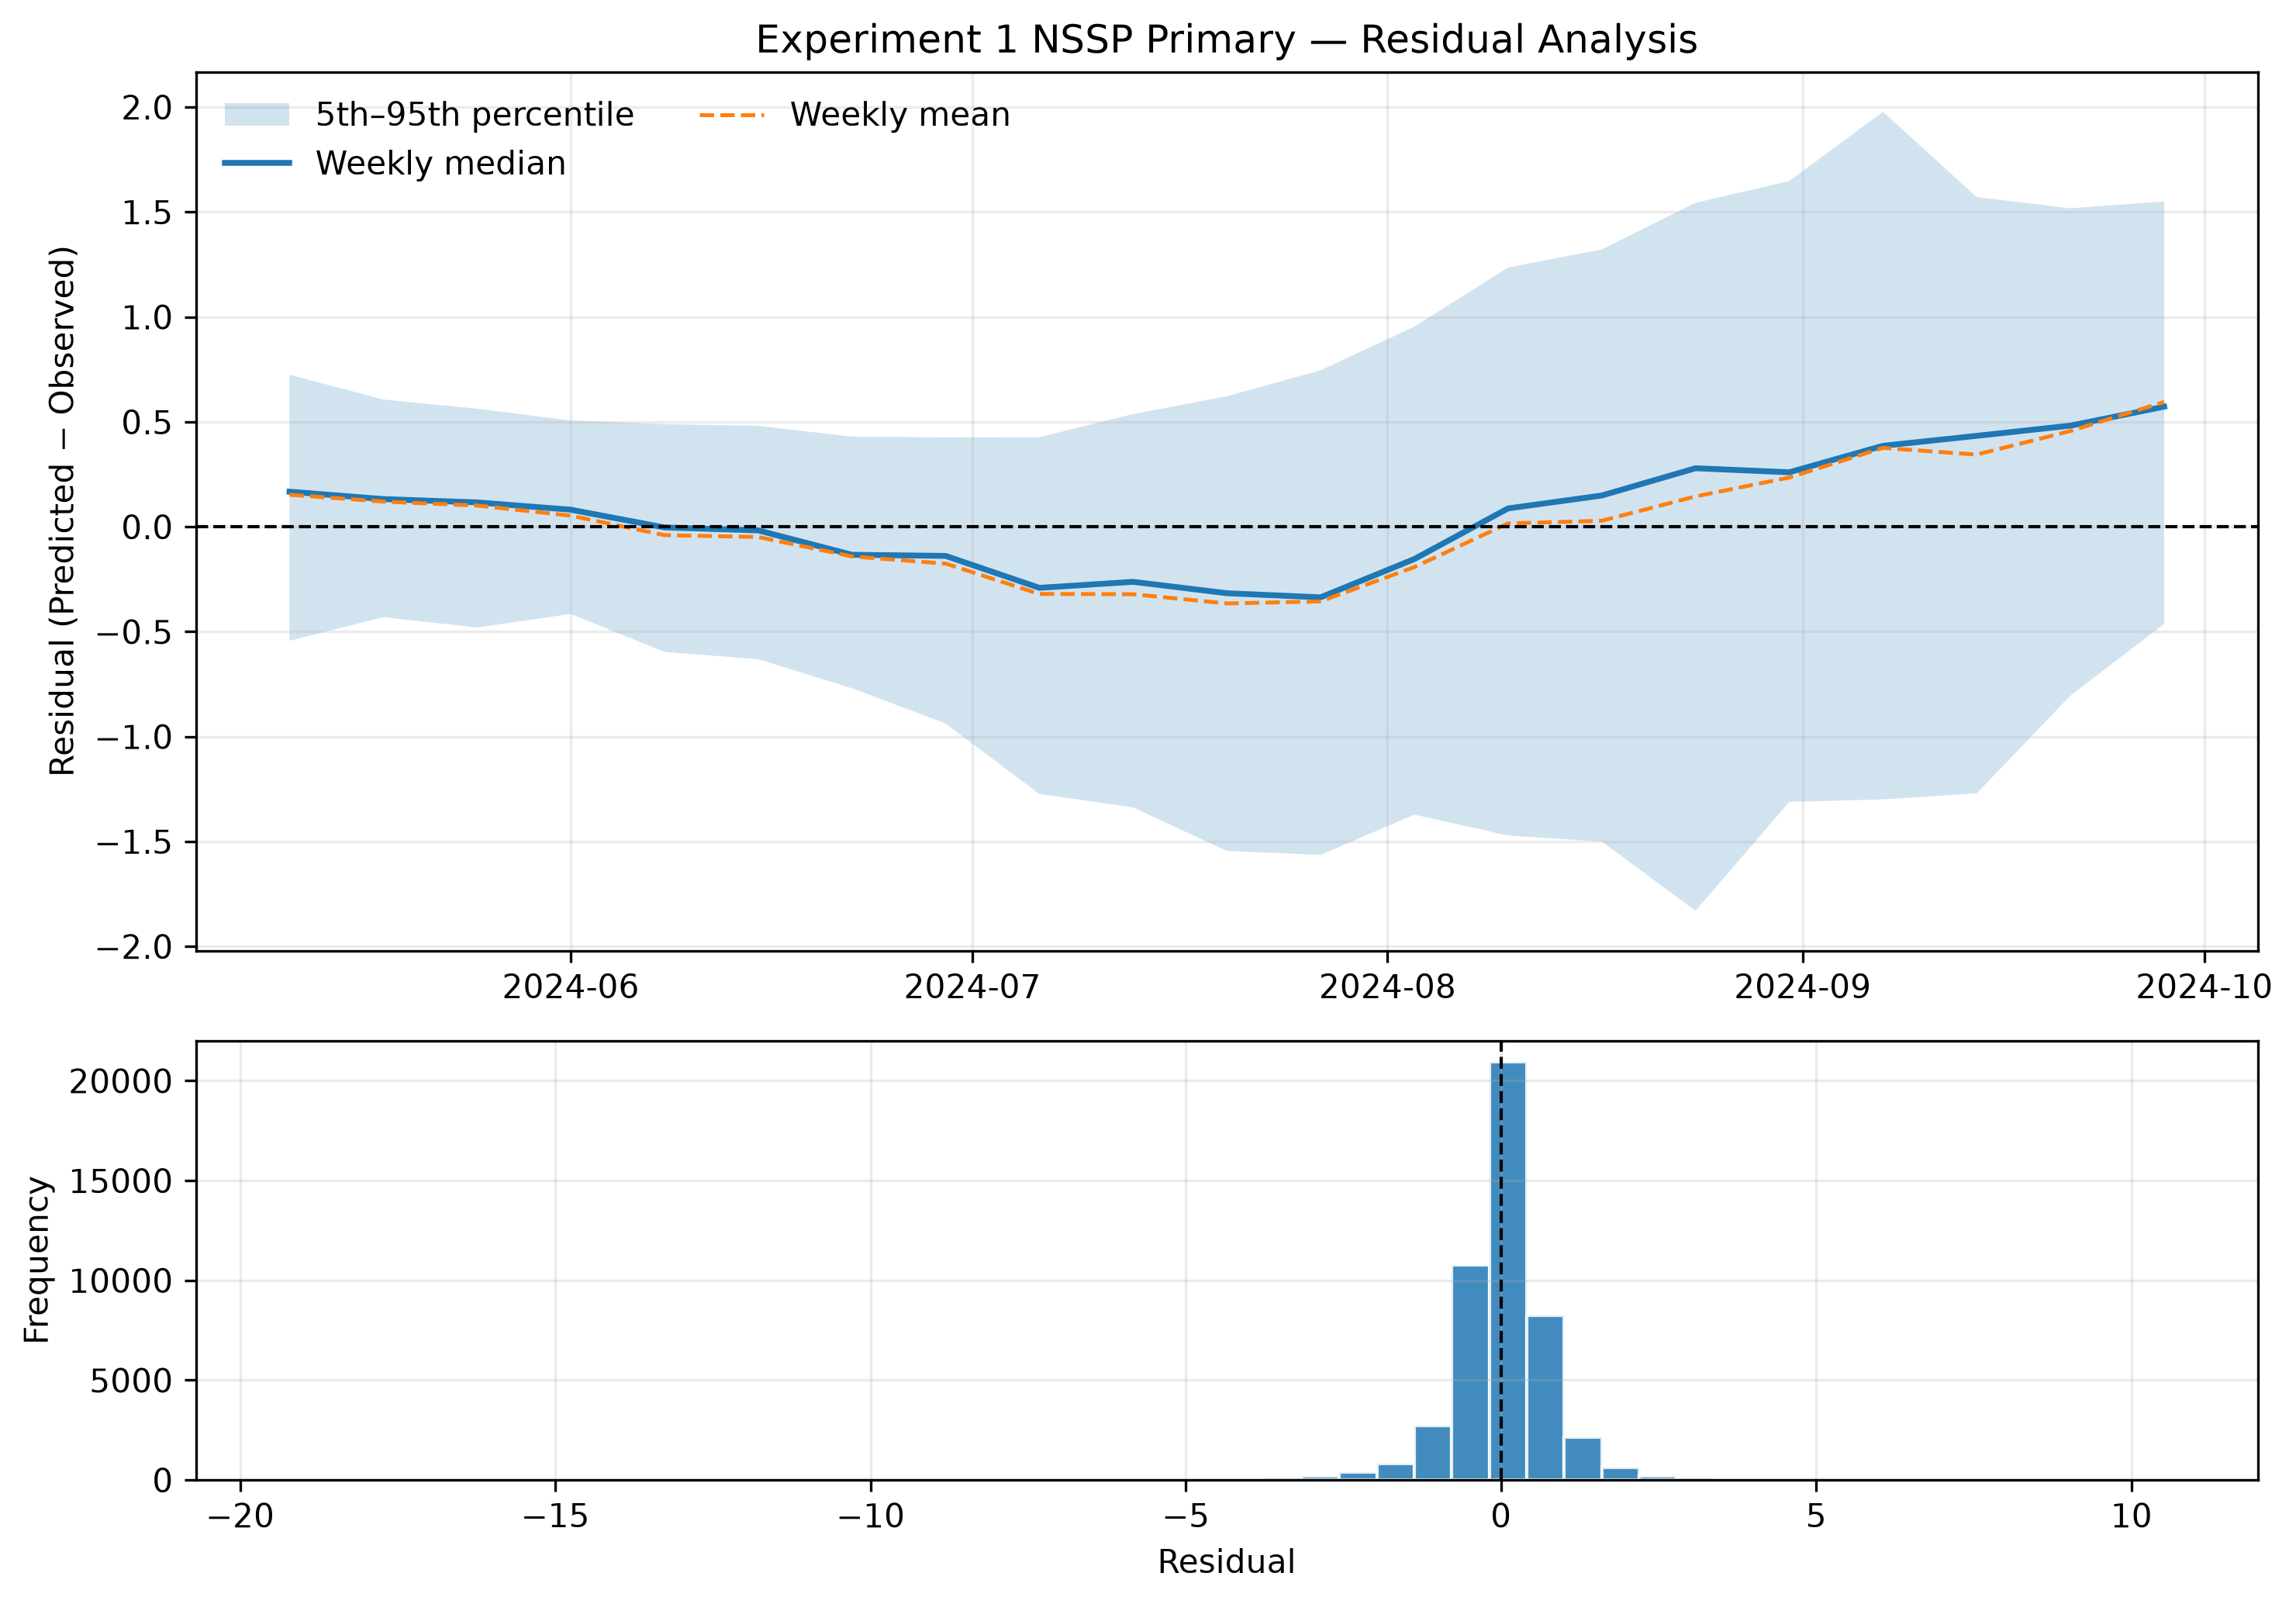
\includegraphics[width=0.74\textwidth]{fig06.png}
\caption{NSSP residual diagnostics across 47,534 held-out reporting-record-week rows and 21 weeks. Errors broaden during the seasonal rise and decline. Repeated HSA assignments contribute to these pooled summaries.}
\label{fig:resid1}
\end{figure}

\begin{figure}[!ht]
\centering
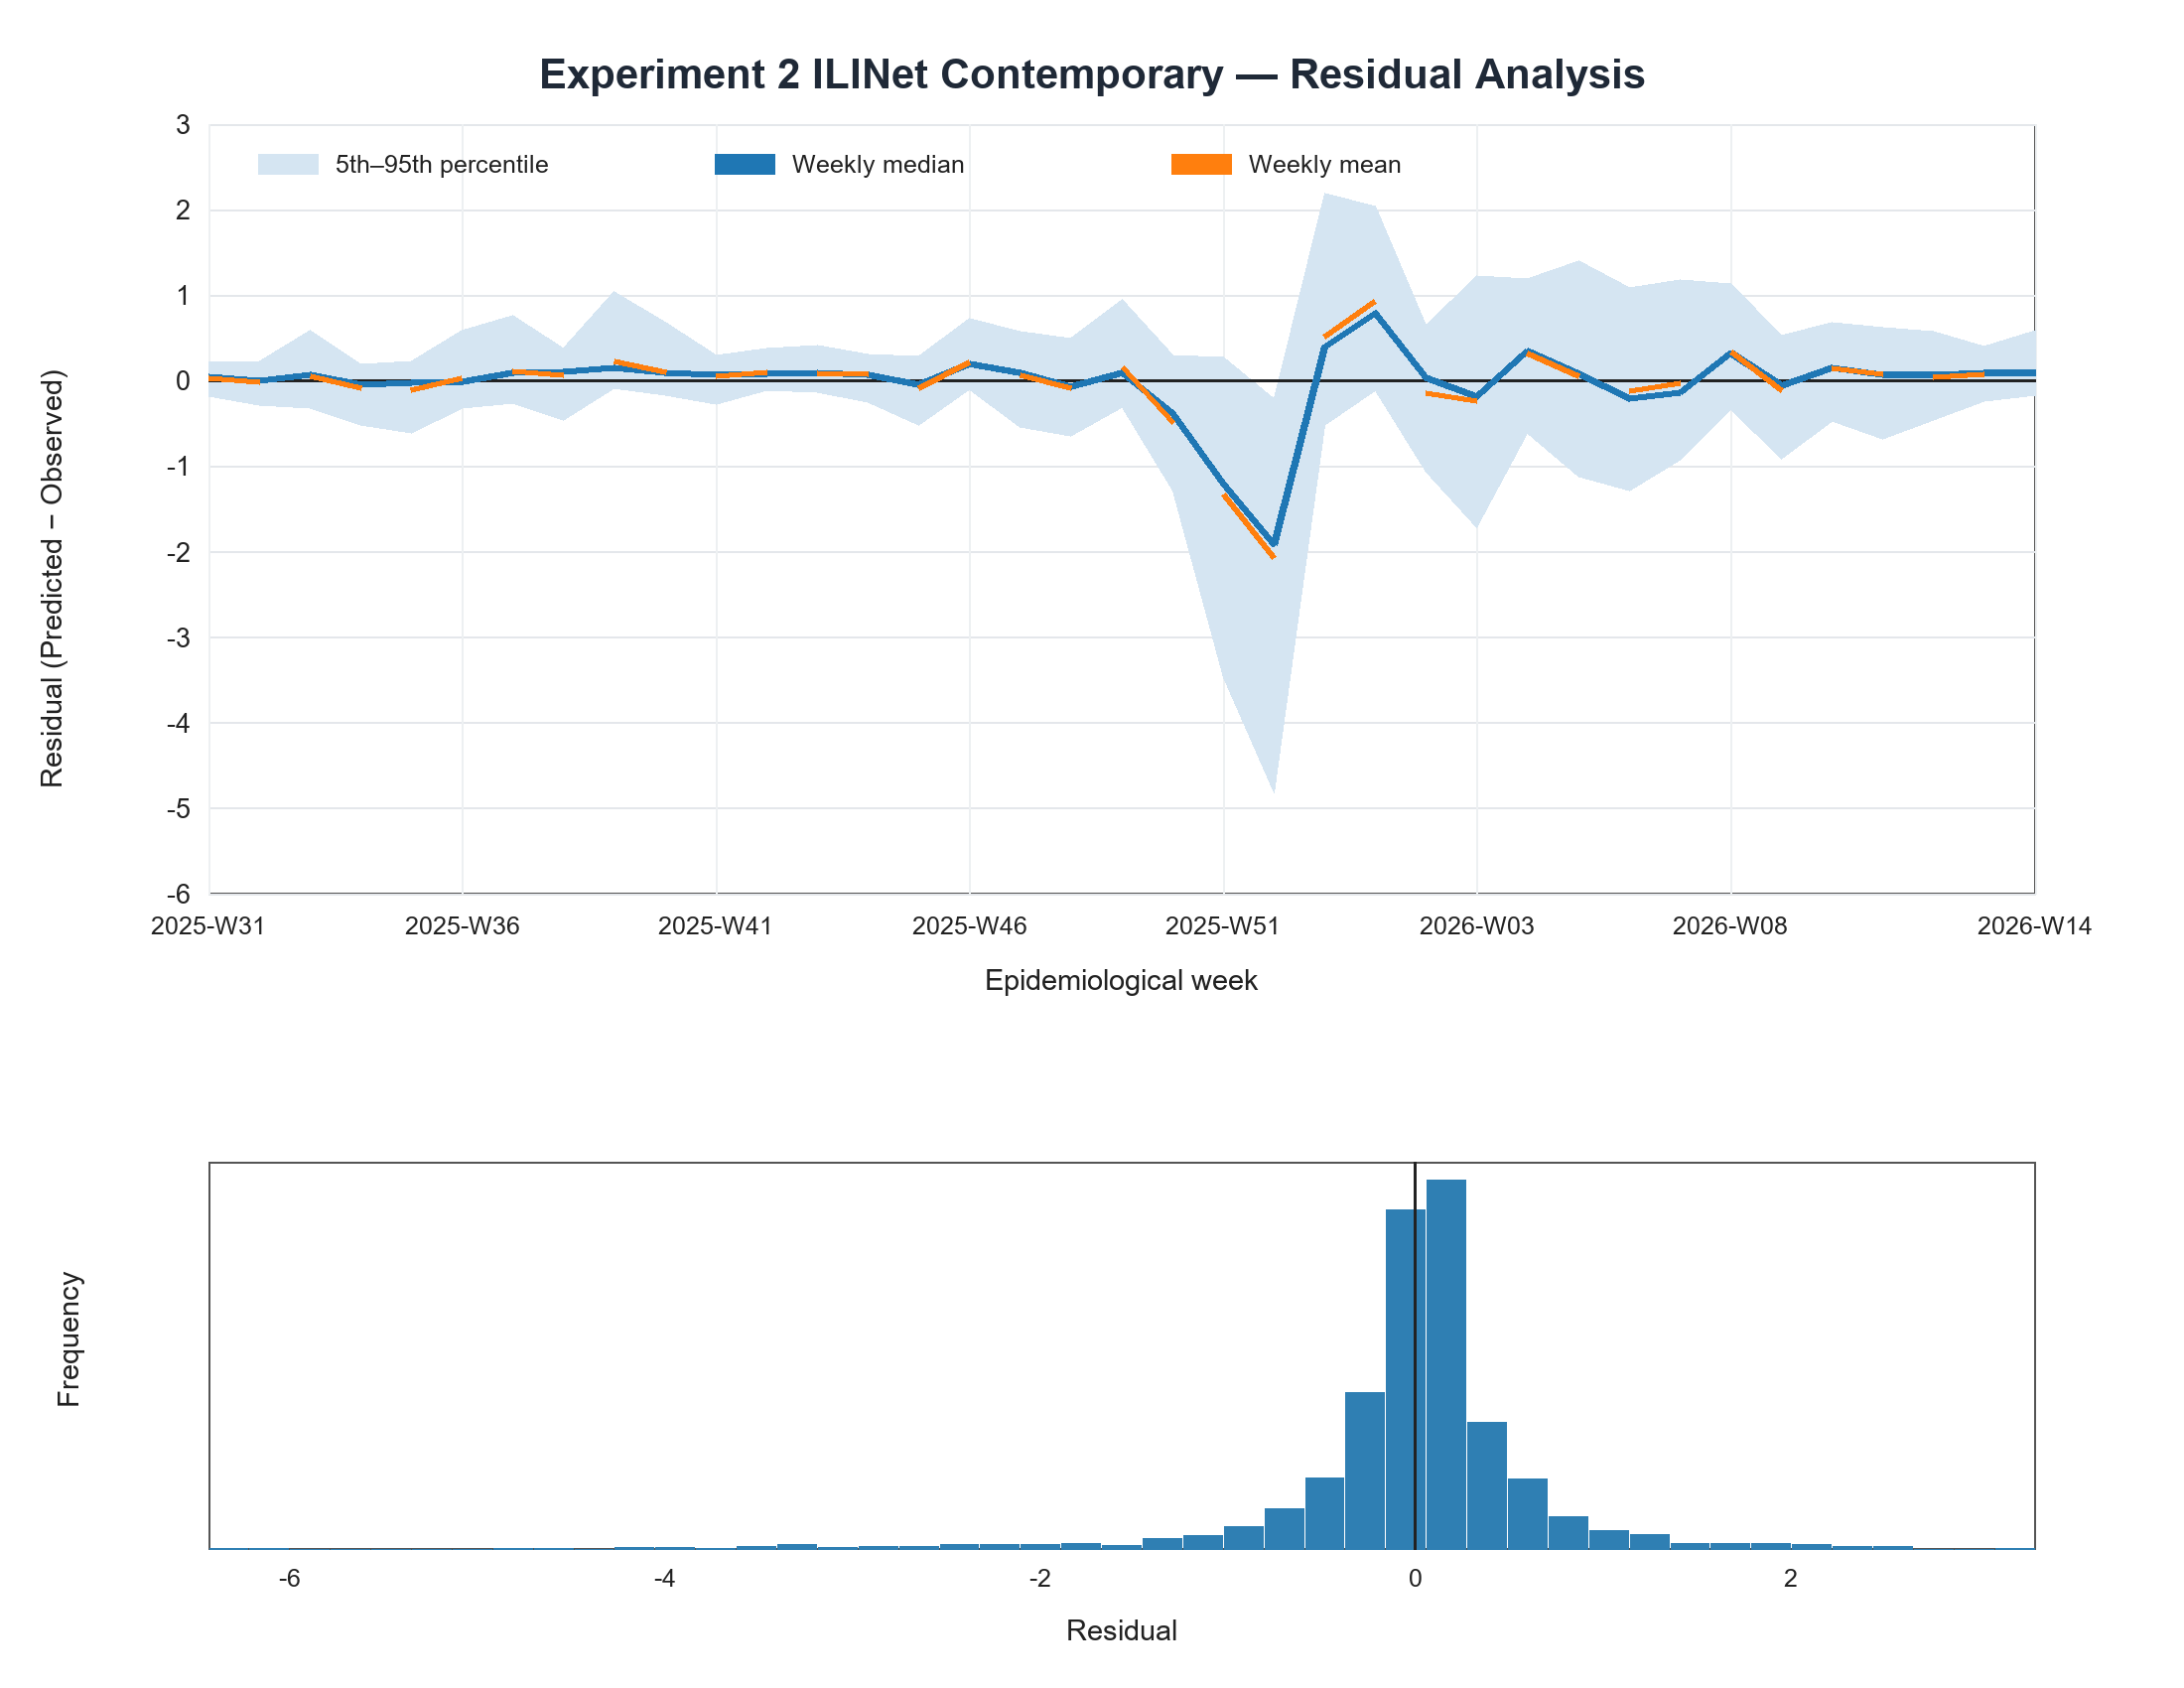
\includegraphics[width=0.74\textwidth]{fig09.png}
\caption{Contemporary ILINet residual diagnostics across all 1,774 test rows and 37 source surveillance weeks, including valid 2025-W53. Week-specific errors near the peak are larger than suggested by the small overall mean bias.}
\label{fig:resid2}
\end{figure}

\clearpage
\begin{figure}[!ht]
\centering
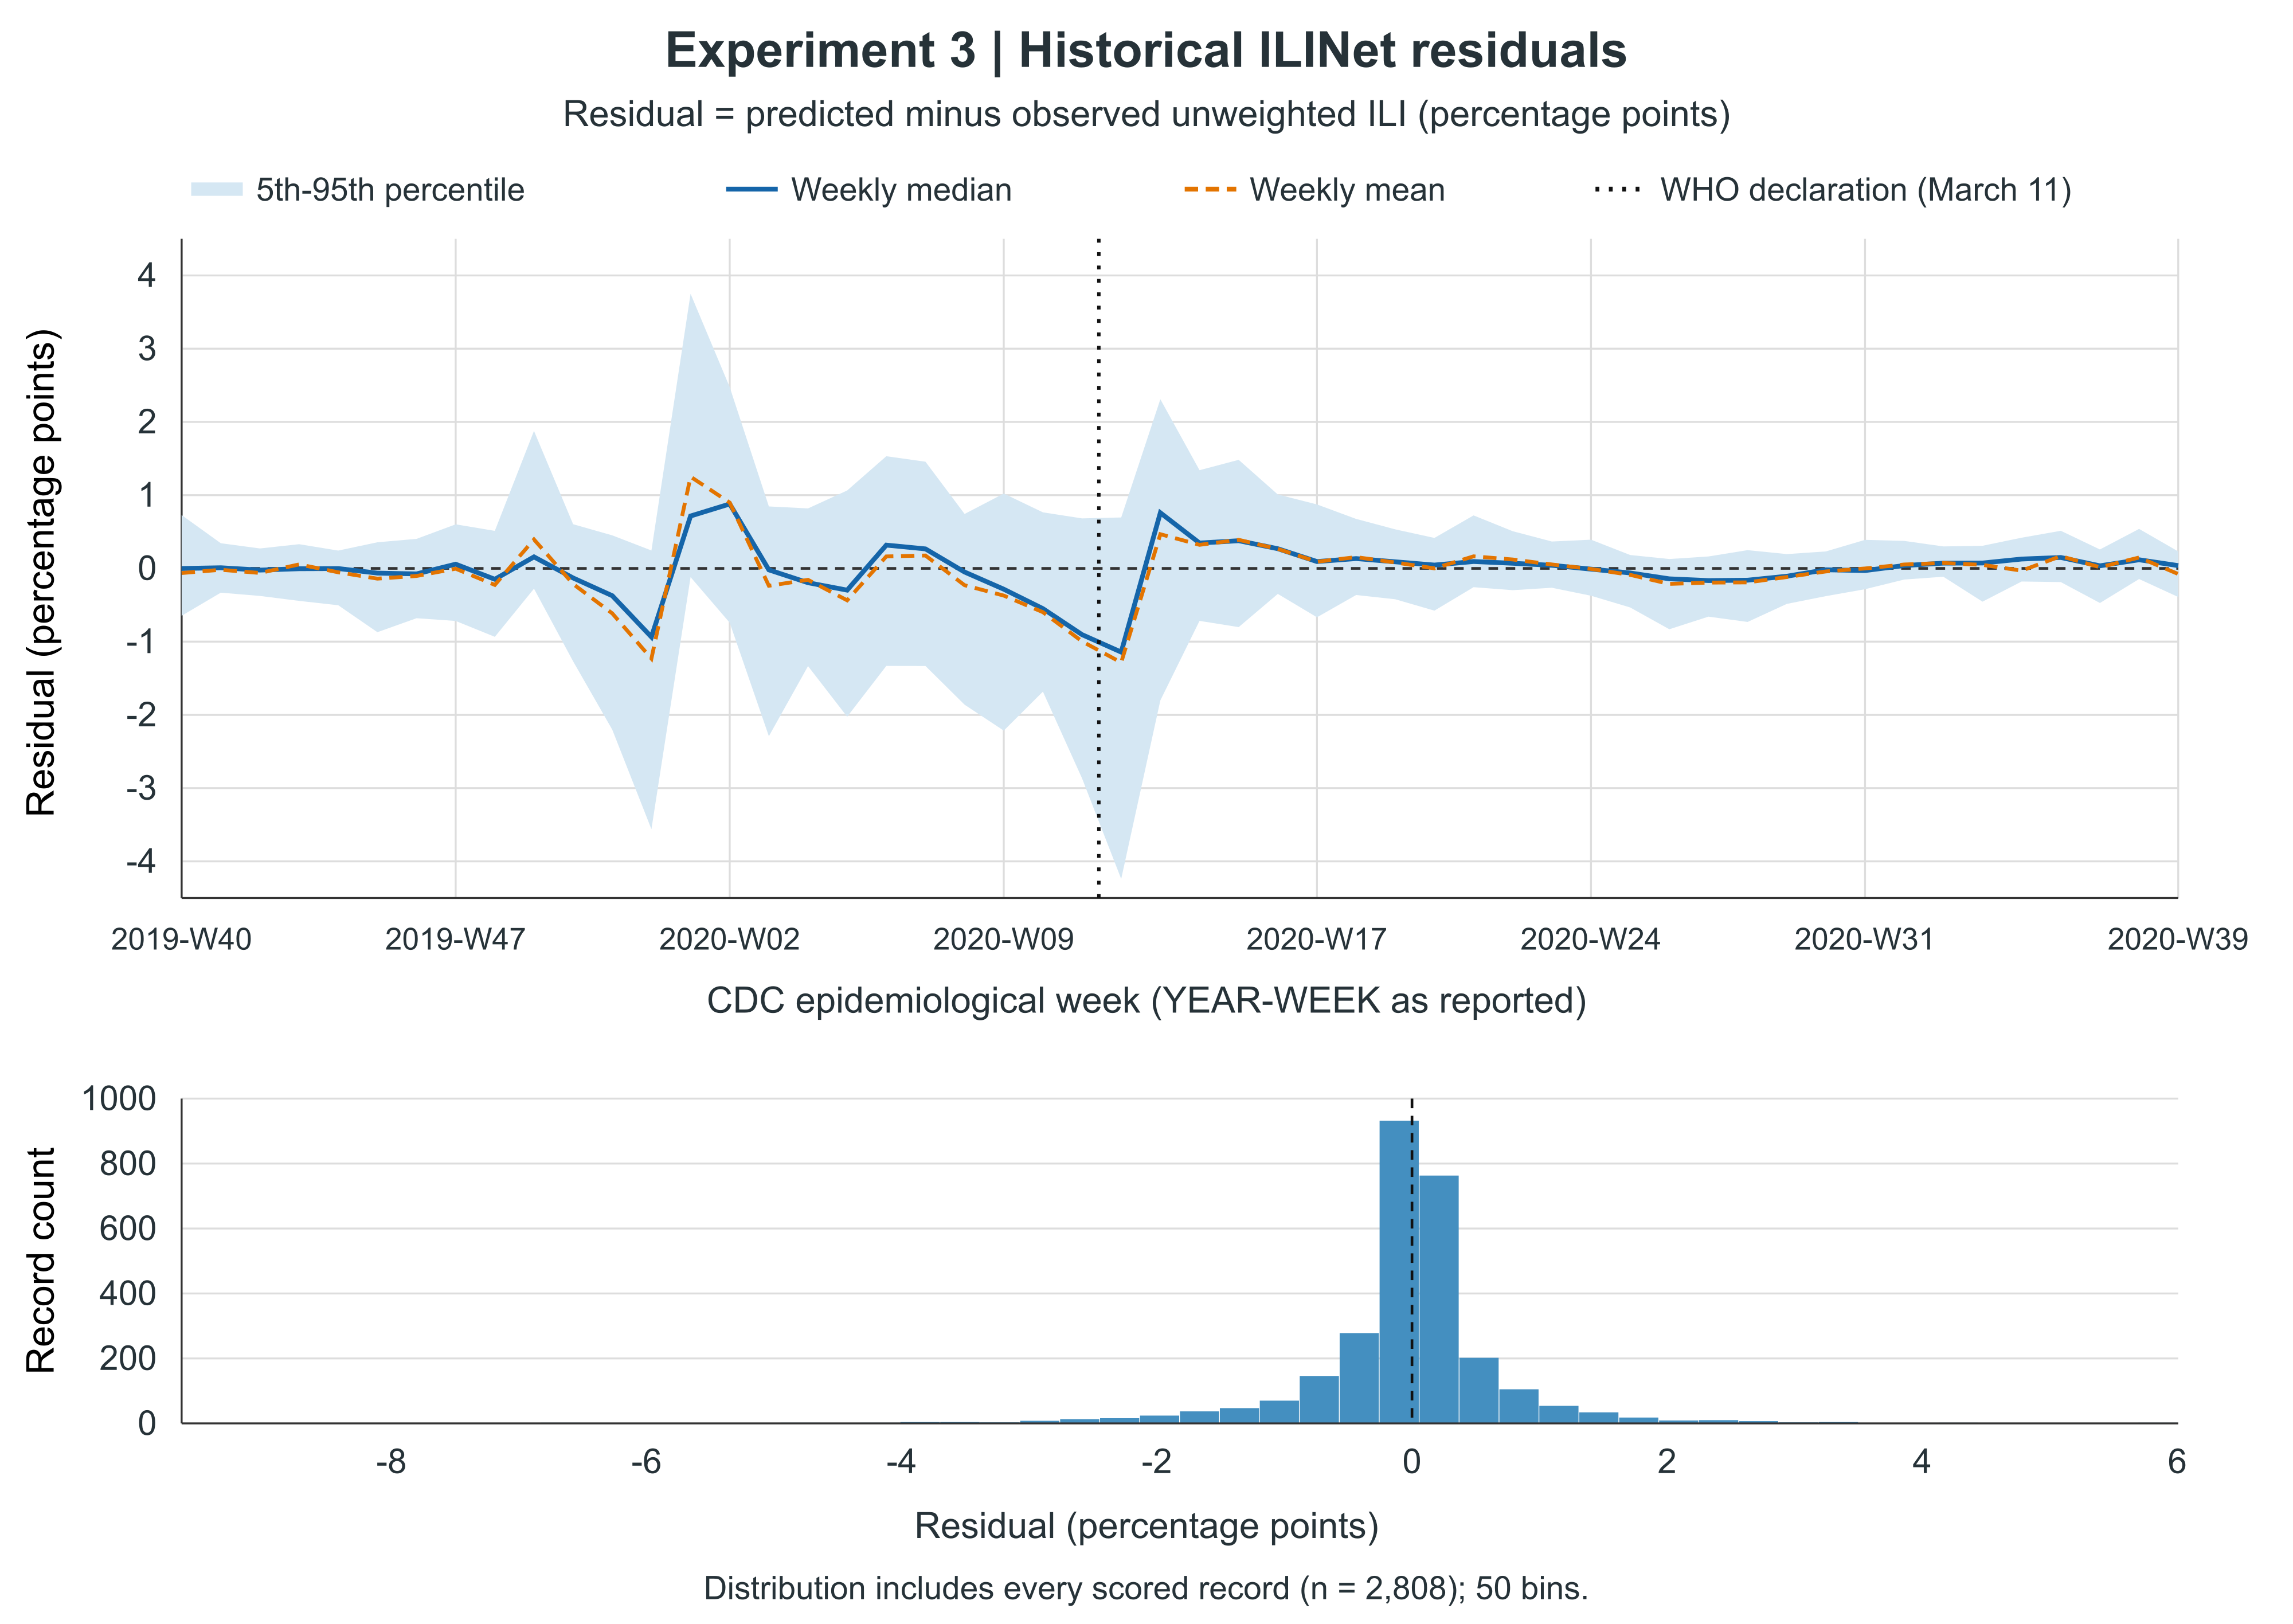
\includegraphics[width=0.90\textwidth]{fig12.png}
\caption{Historical ILINet residual diagnostics across 2,808 test rows and 52 source weeks. The March 11, 2020 WHO pandemic declaration \cite{who} is a descriptive marker. Week-start grouping places March 8--14 in the group beginning before the declaration; this is not a causal boundary.}
\label{fig:resid3}
\end{figure}

The original record-weighted mean residual is +0.031 percentage points for NSSP; primary HSA-week scoring gives +0.035. ILINet means remain -0.019 and -0.047 for the contemporary and historical experiments. Small aggregate biases do not rule out larger week-specific errors or delayed peaks. The historical residual distribution narrows during later low-burden months; lower MAE/RMSE in that interval does not imply better performance at turning points. No residual figure or model fit was changed for this reporting amendment.

\section*{S6. Full-size geographic maps}
\label{sec:S6}
Figures~\ref{fig:map1}--\ref{fig:map3} reproduce the three unchanged map assets at larger size. They summarize mean held-out predictions, not peak-week burden. Orange NSSP uses a target-specific 0--4\% scale; blue and purple ILINet maps share 0--6\% limits. Darker shades indicate higher mean predicted percentages; gray indicates missing eligible mapped data, not zero burden. Alaska and Hawaii are insets.

NSSP state summaries average included within-state records and weeks, including repeated HSA assignments and available state aggregates. They are not official state estimates or population-weighted rates. ILINet polygons use each state's own series; New York City, Puerto Rico, and the Virgin Islands remain separate in companion data. No map tests spatial dependence, density associations, causal effects, or hotspot-classification accuracy. \nolinkurl{map_values.csv} supplies row counts, week coverage, observed/predicted means, and bias; \nolinkurl{map_provenance.json} records sources and hashes.

\clearpage
\begin{figure}[!ht]
\centering
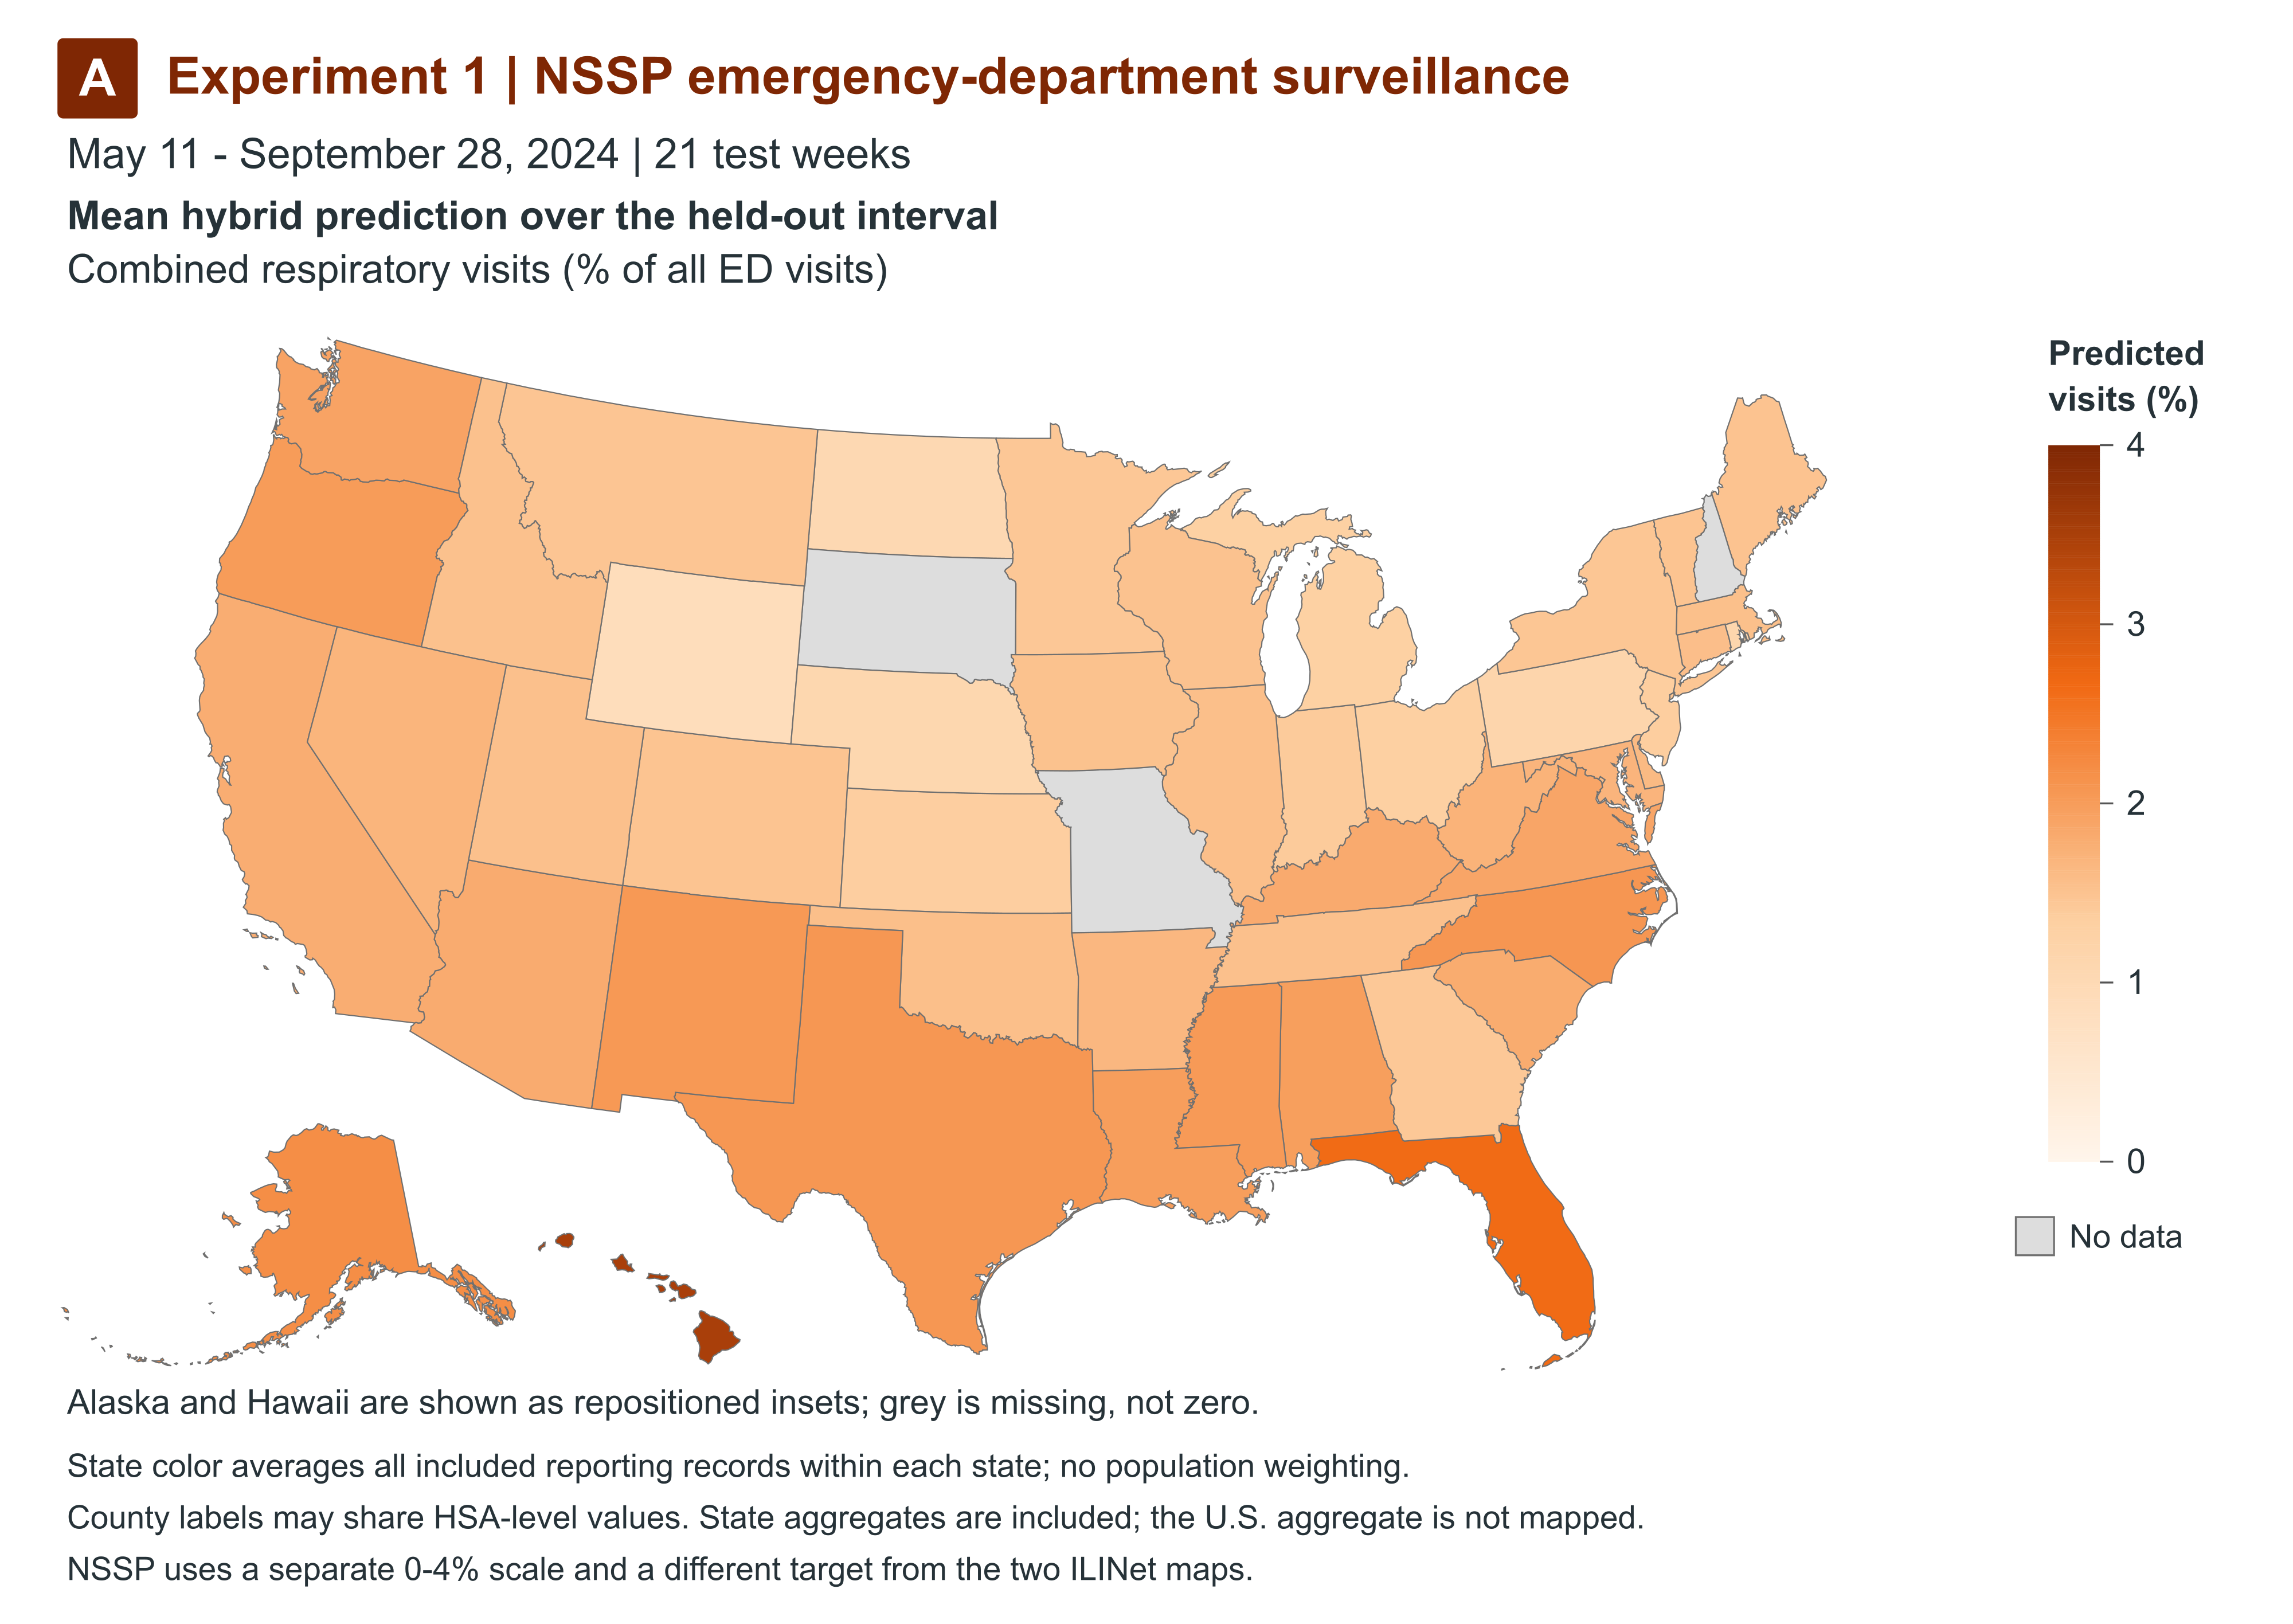
\includegraphics[width=\textwidth]{fig13.png}
\caption{Experiment 1: NSSP mean predicted respiratory ED-visit percentage, May 11--September 28, 2024. These are reporting-record-weighted within-state averages under the included cohort, not official statewide rates.}
\label{fig:map1}
\end{figure}

\clearpage
\begin{figure}[!ht]
\centering
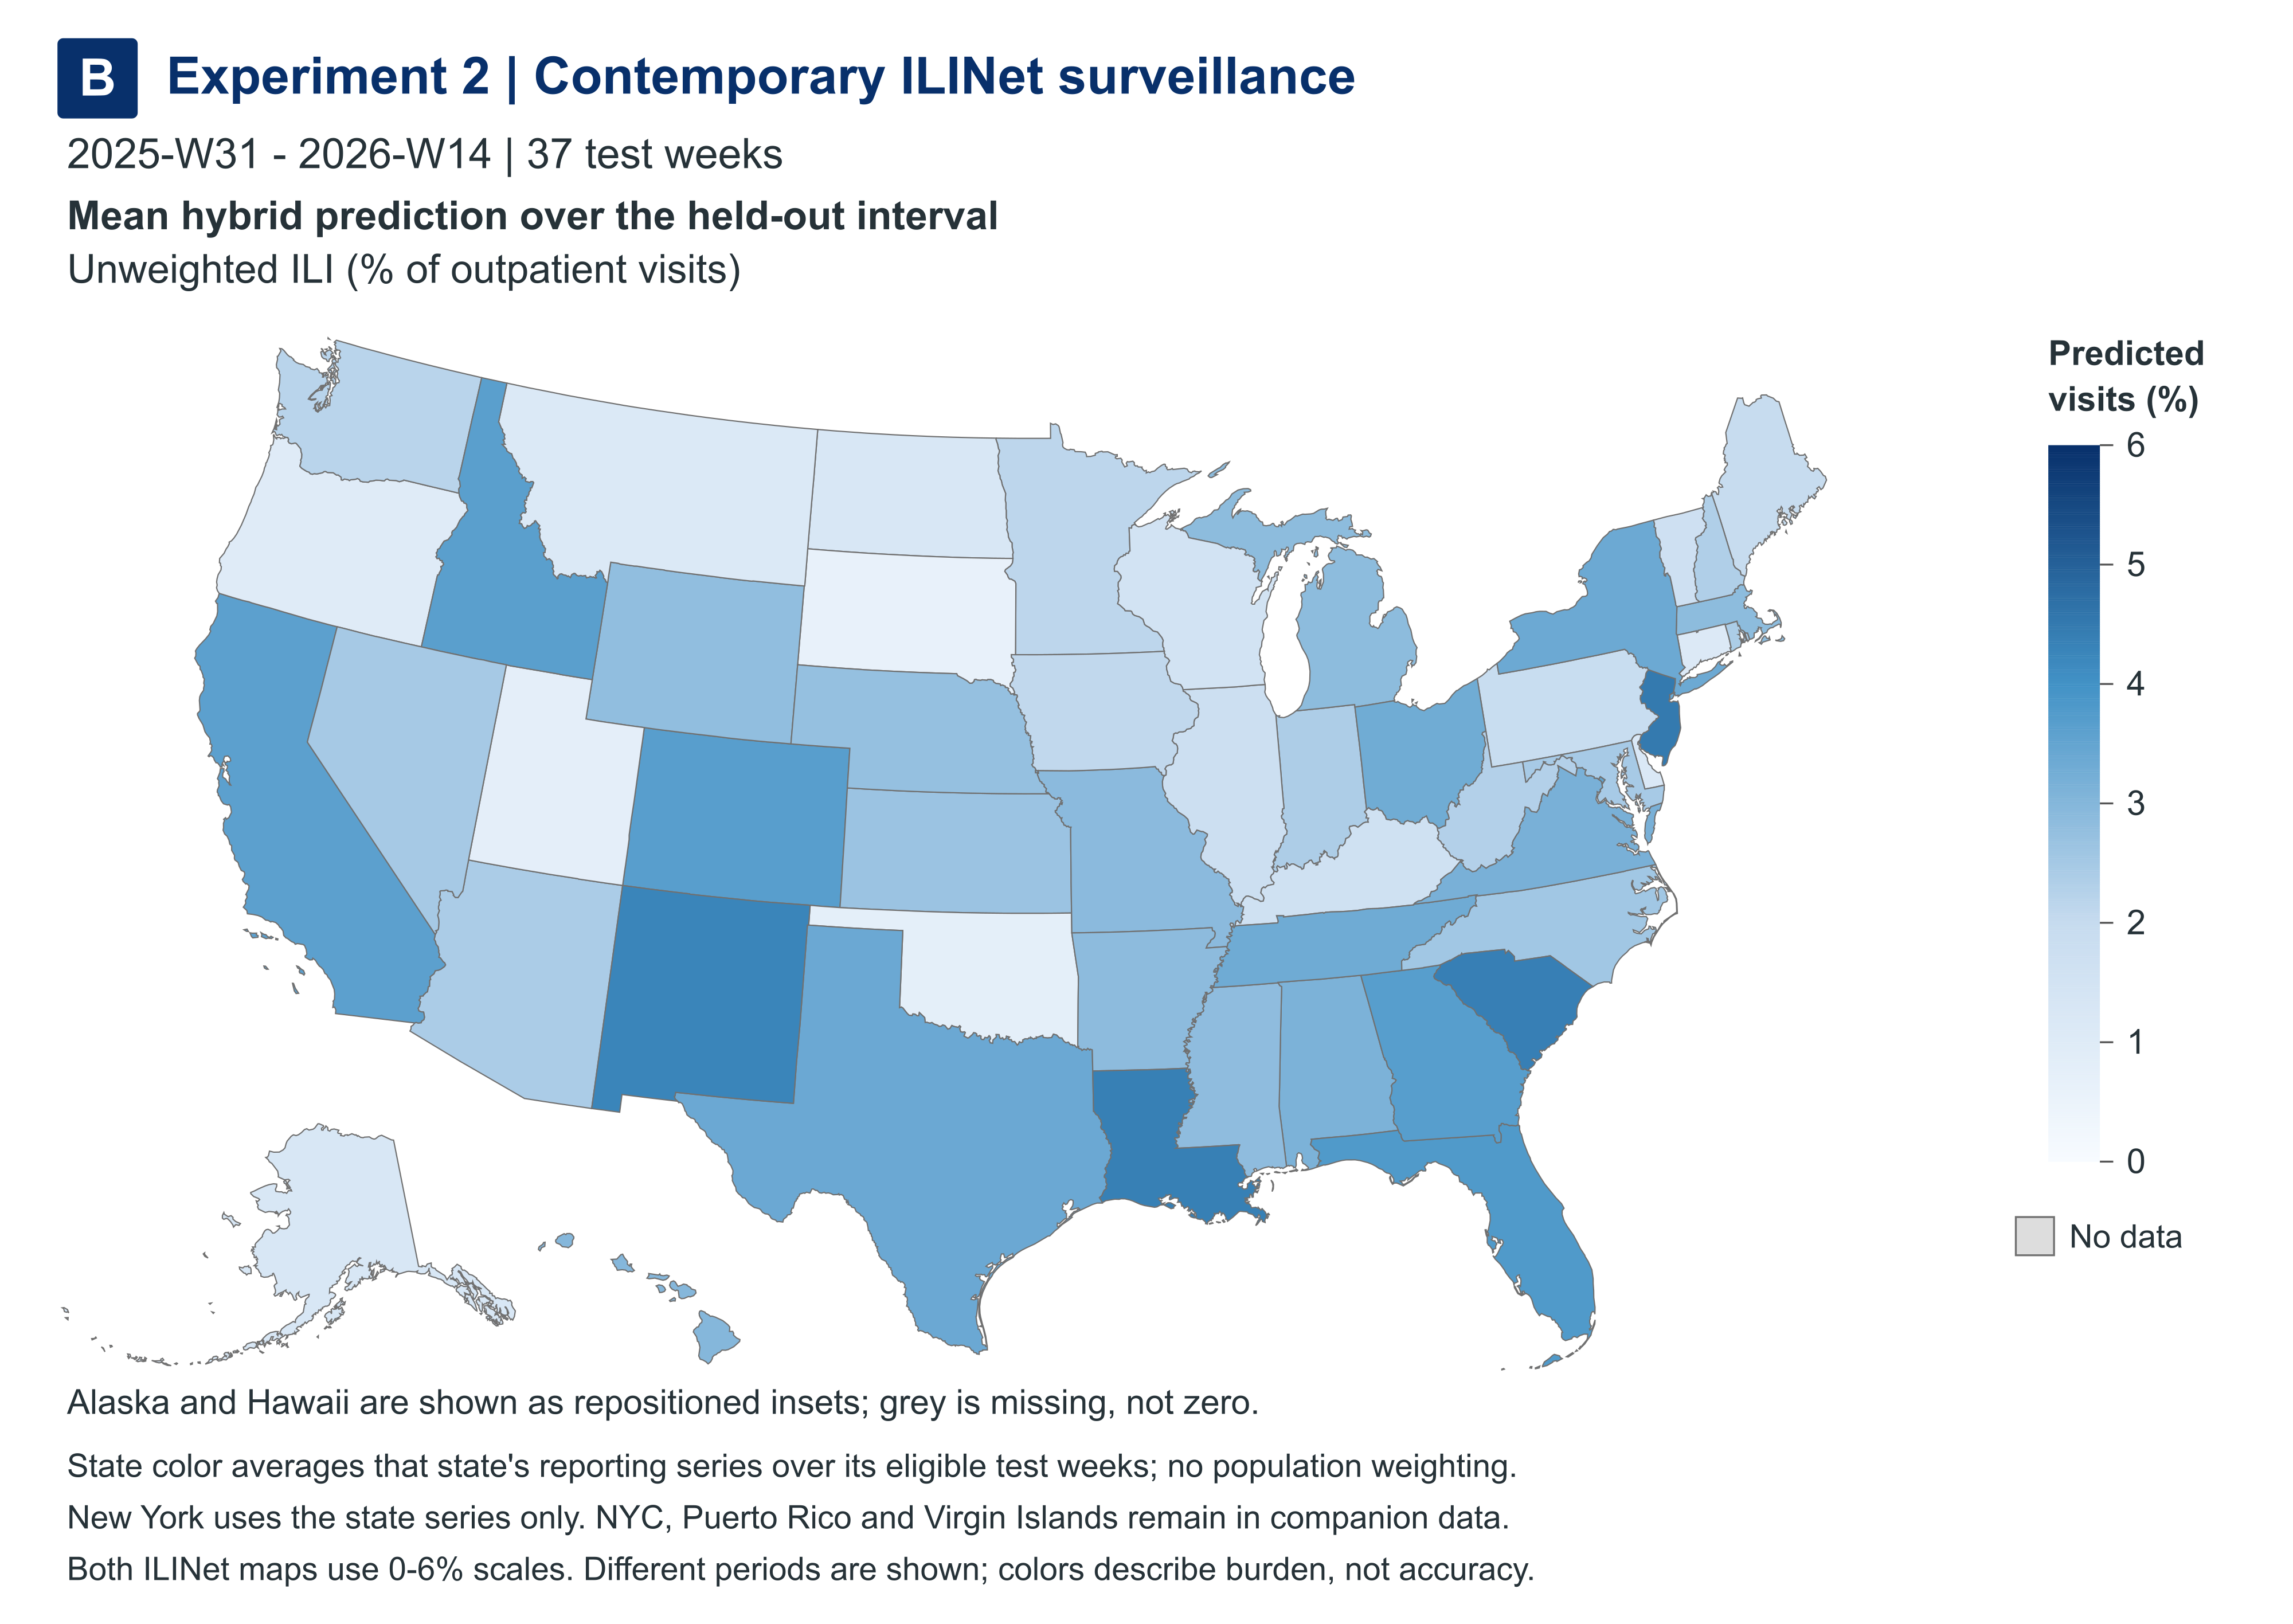
\includegraphics[width=\textwidth]{fig14.png}
\caption{Experiment 2: contemporary ILINet mean predicted unweighted ILI percentage, 2025-W31--2026-W14. Each polygon uses the state's own eligible reporting series. The numerical limits match the historical ILINet map; colors distinguish the experiments.}
\label{fig:map2}
\end{figure}

\clearpage
\begin{figure}[!ht]
\centering
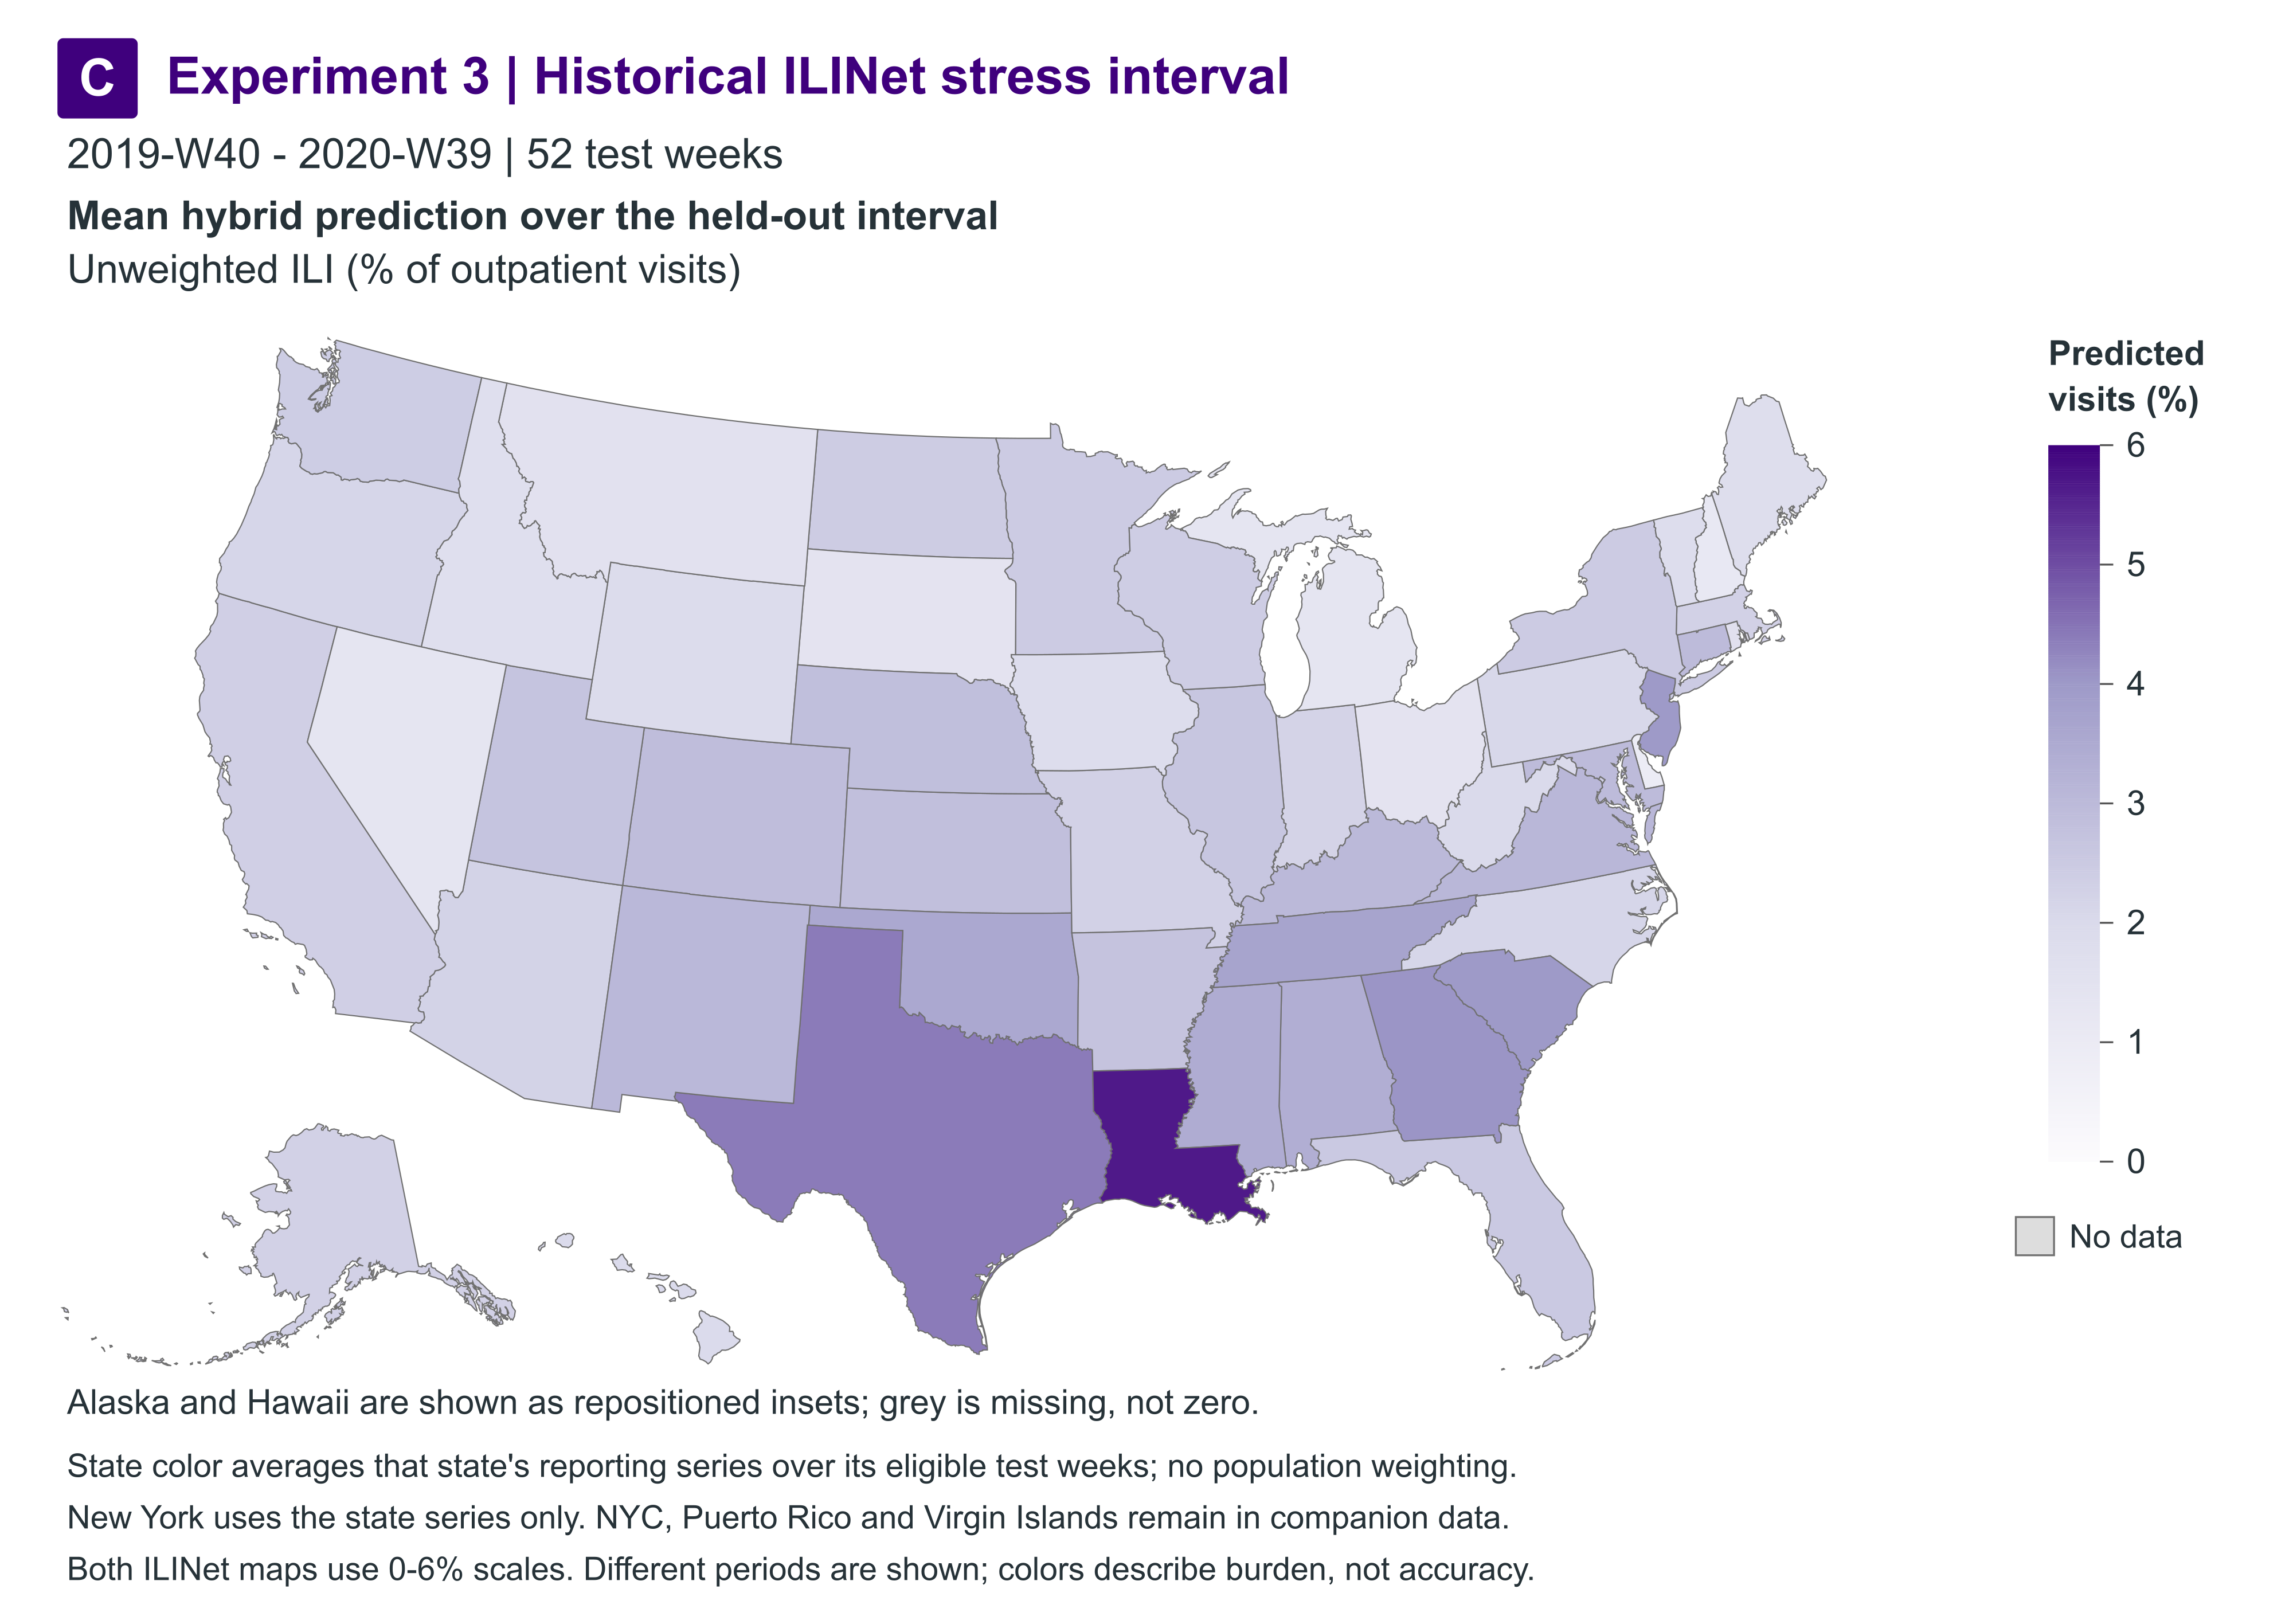
\includegraphics[width=\textwidth]{fig15.png}
\caption{Experiment 3: historical ILINet mean predicted unweighted ILI percentage, 2019-W40--2020-W39. Comparisons with the contemporary ILINet map are descriptive because the test periods differ. Gray means no eligible mapped data.}
\label{fig:map3}
\end{figure}

\clearpage
\section*{S7. Observed and predicted temporal trajectories}
\label{sec:S7}
The unchanged plots below show weekly means across eligible reporting records. NSSP trajectories and residual figures retain the original record weighting, distinct from primary HSA-week scoring. ILINet metrics continue to use reporting-unit-week rows. These plots are descriptive and do not replace the defined scoring units.

\begin{figure}[!ht]
\centering
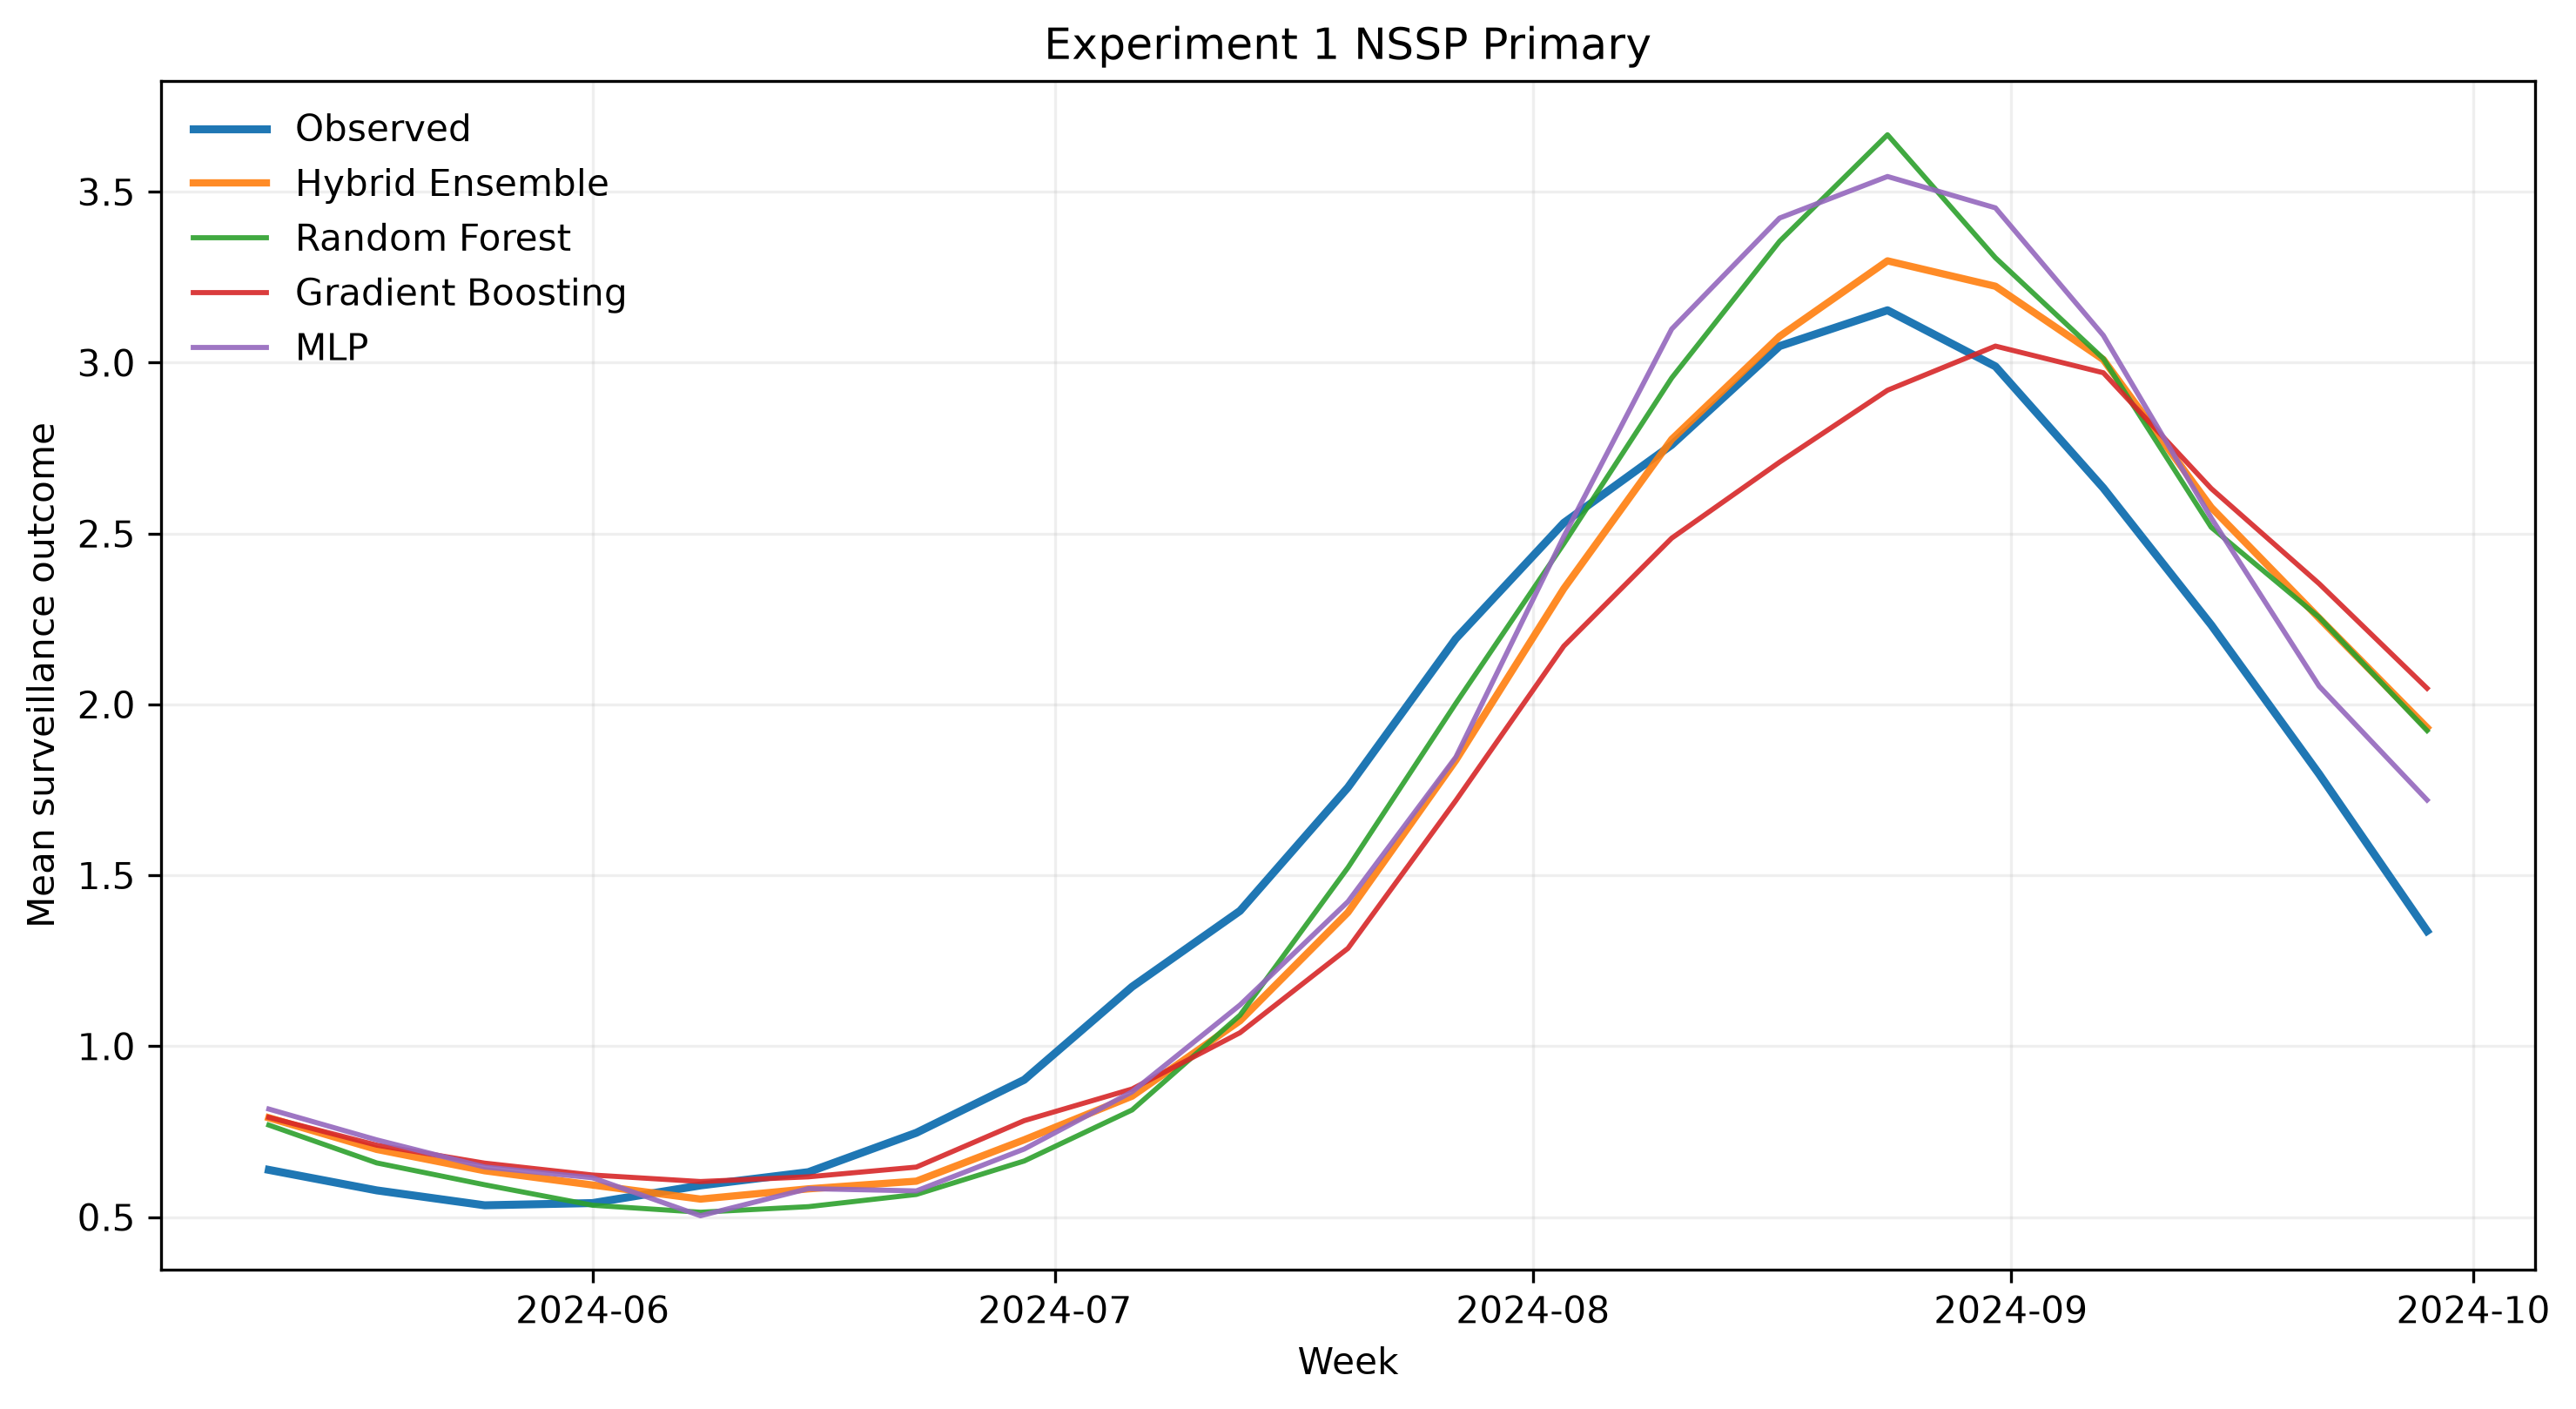
\includegraphics[width=0.95\textwidth]{fig04.png}
\caption{NSSP observed and predicted weekly mean combined respiratory ED-visit percentage over 21 final-test weeks. The curves summarize the 47,534 eligible reporting-record-week rows. Observed and hybrid means peak on August 24, 2024; the hybrid overpredicts that weekly maximum by 0.145 percentage points.}
\label{fig:trajectory1}
\end{figure}

\begin{figure}[!ht]
\centering
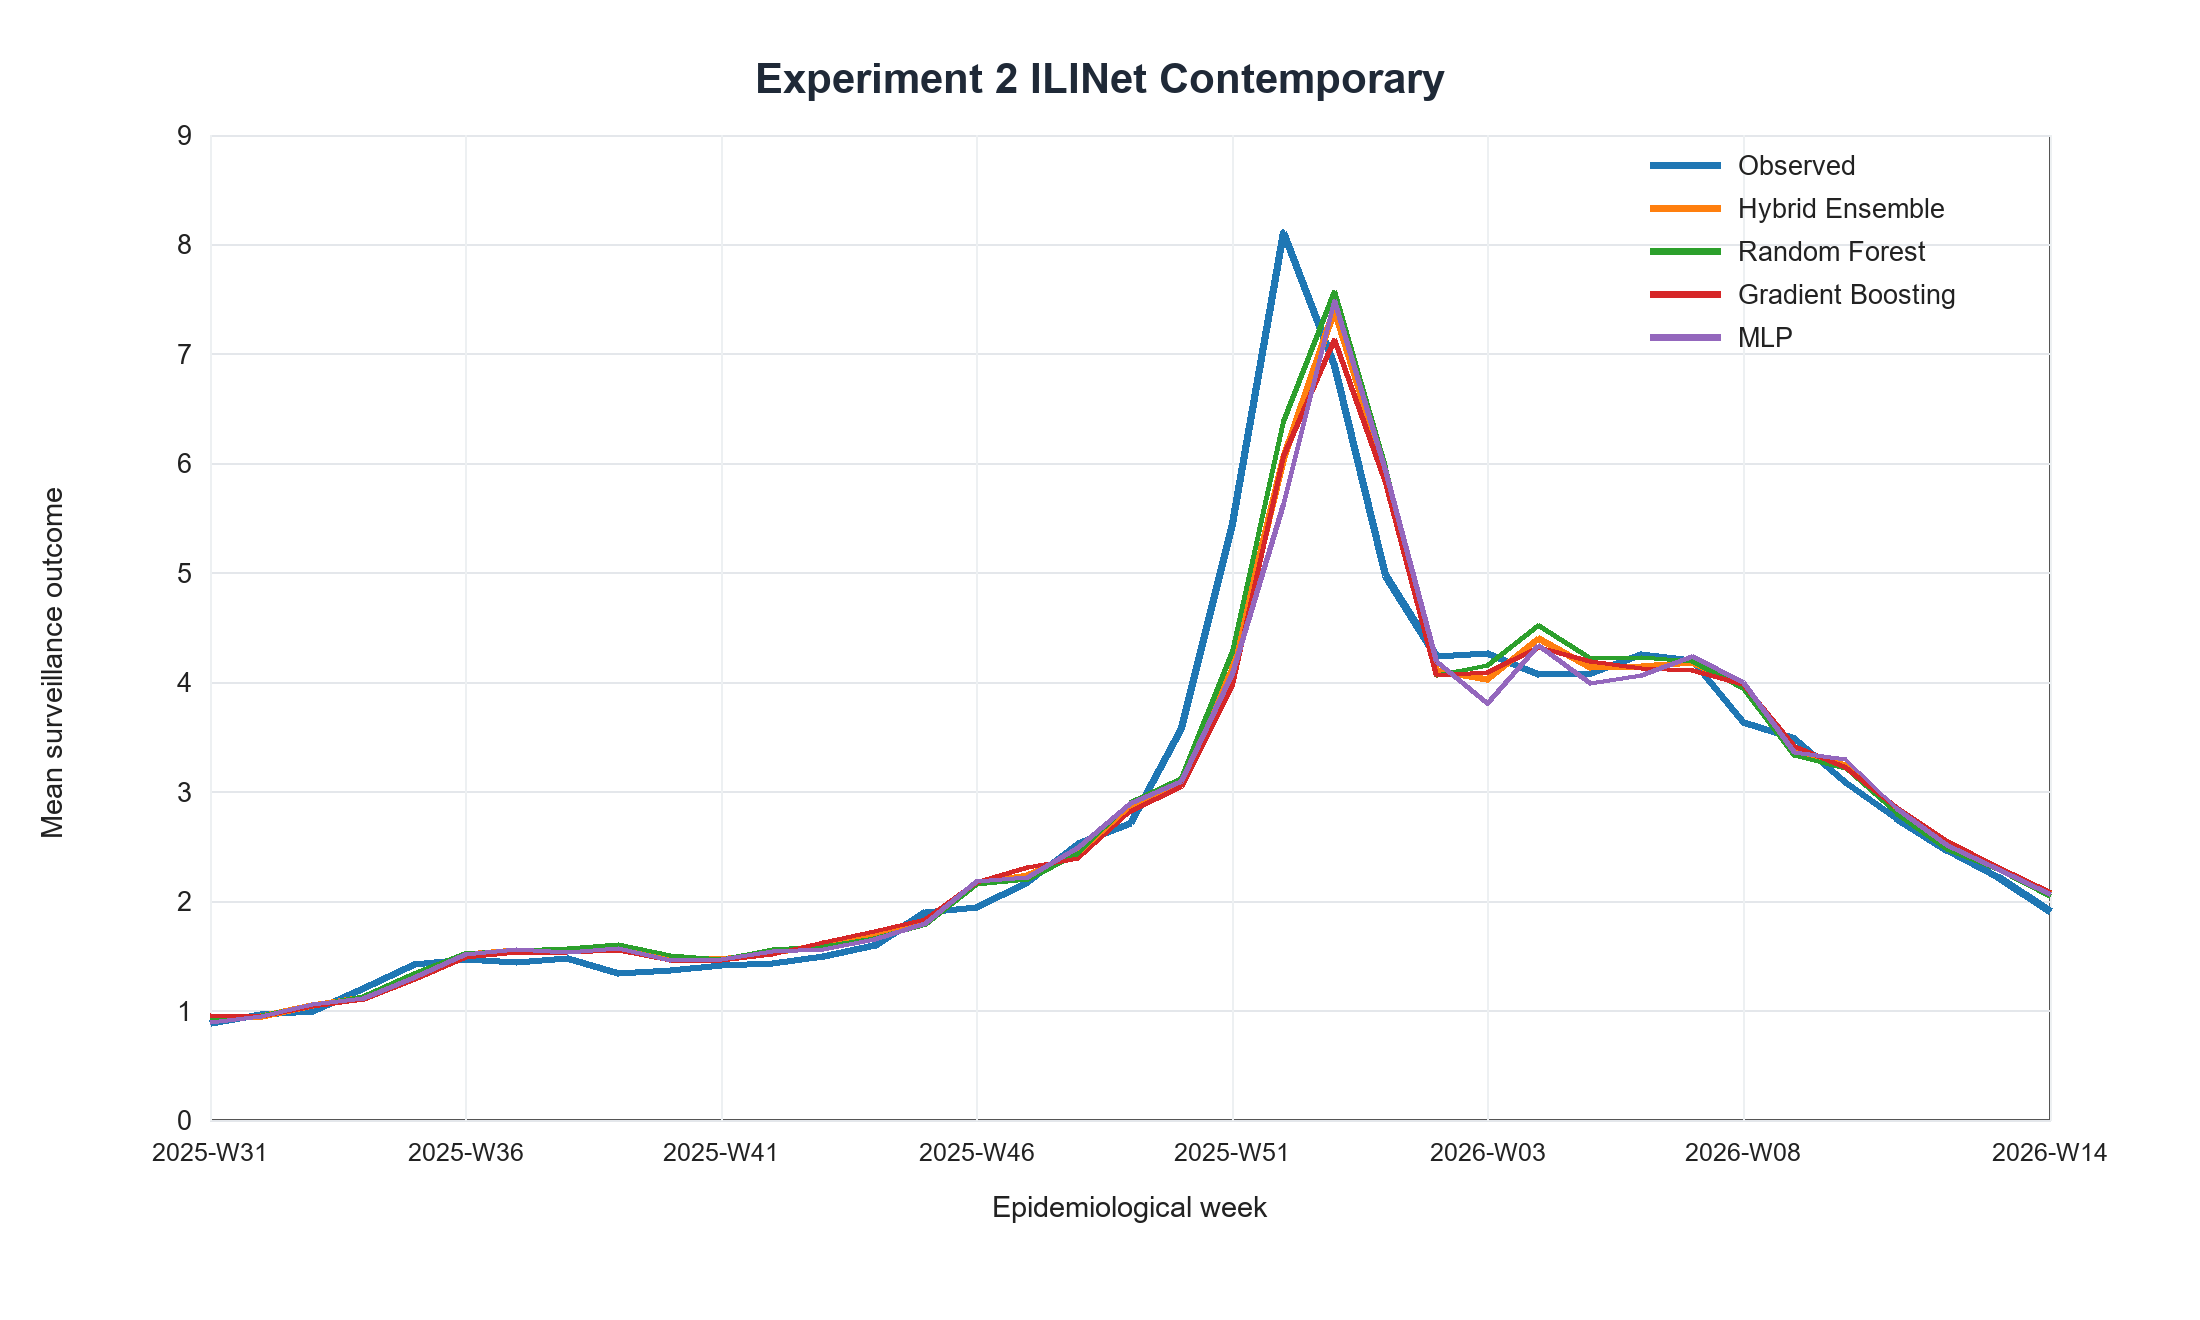
\includegraphics[width=0.95\textwidth]{fig07.png}
\caption{Contemporary ILINet observed and predicted weekly mean unweighted ILI over 37 surveillance weeks, including valid 2025-W53. Metrics use all 1,774 eligible rows. The observed weekly maximum is 8.112\% in 2025-W52; the hybrid maximum is 7.403\% in 2025-W53, one surveillance week later.}
\label{fig:trajectory2}
\end{figure}

\clearpage
\begin{figure}[!ht]
\centering
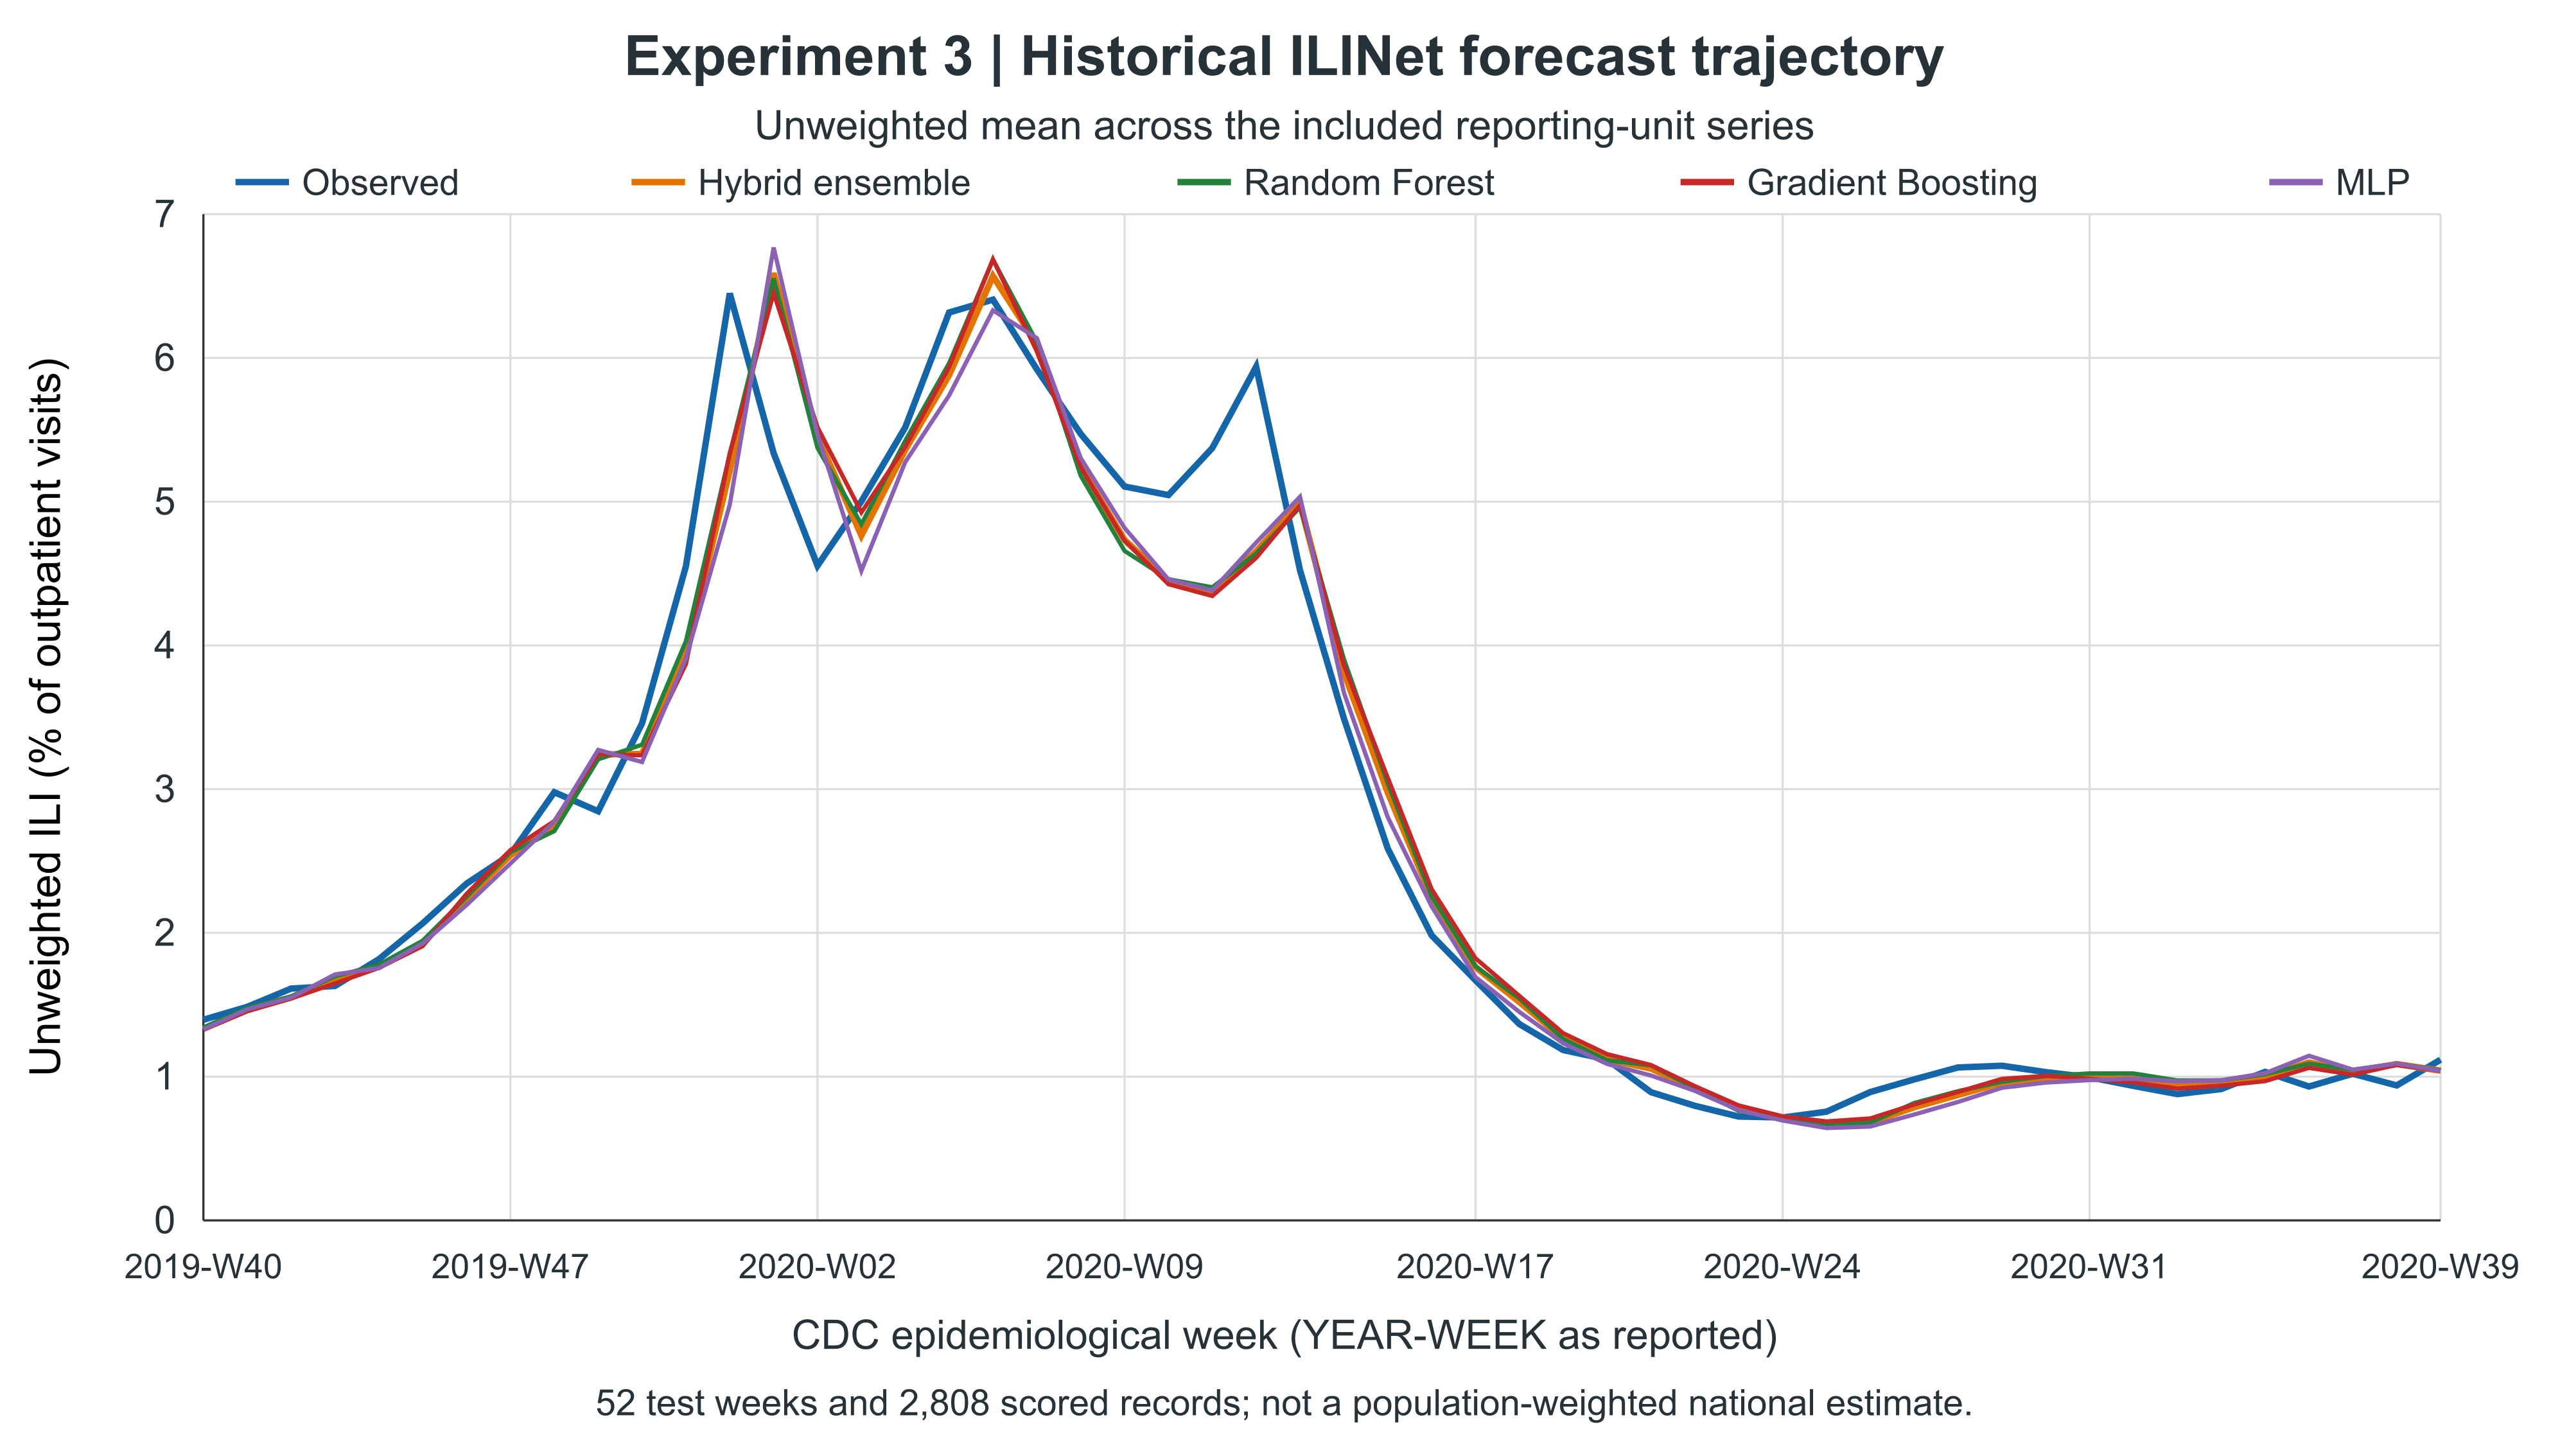
\includegraphics[width=\textwidth]{fig10.png}
\caption{Historical ILINet observed and predicted weekly mean unweighted ILI over 52 final-test weeks. Metrics use all 2,808 eligible rows. The observed maximum is 6.449\% in 2019-W52; the hybrid maximum is 6.589\% in 2020-W01, one surveillance week later.}
\label{fig:trajectory3}
\end{figure}

\begin{thebibliography}{S1}
\bibitem[S1]{who} World Health Organization, ``WHO Director-General's opening remarks at the media briefing on COVID-19---11 March 2020,'' Mar. 11, 2020. [Online]. Available: \url{https://www.who.int/news-room/speeches/item/who-director-general-s-opening-remarks-at-the-media-briefing-on-covid-19---11-march-2020}. Accessed: Nov. 14, 2026.
\end{thebibliography}

\vfill
\noindent\textbf{AI-assisted preparation.} OpenAI ChatGPT/Codex assisted the organization and wording of Sections S1--S7, LaTeX presentation, and the archived supporting code/documentation. Figures reproduce recorded surveillance data and model outputs, not AI-synthesized observations. The authors are responsible for the calculations, interpretation, citations in the companion paper, and submitted content.
\end{document}
